% -*- mode: LaTeX; coding: utf-8 -*-
\documentclass[12pt]{article}
\usepackage[unicode,colorlinks]{hyperref}
\usepackage[T2A]{fontenc}
\usepackage[utf8]{inputenc}
\usepackage[russian]{babel}
\usepackage{amsmath}
\usepackage{amssymb}
\usepackage{eufrak}
\usepackage{epsfig}
%\usepackage[mathscr]{eucal}
\usepackage{psfrag}
\usepackage{tabularx}
\usepackage{wrapfig}
%\usepackage{eucal}
\usepackage{euscript}

\usepackage[usenames]{color}
\usepackage{colortbl} 

\definecolor{codegreen}{rgb}{0,0.6,0}
\definecolor{codegray}{rgb}{0.5,0.5,0.5}
\definecolor{codeblack}{rgb}{0.1,0.,0.3}
\definecolor{codeemph}{rgb}{0.5,0.1,0.5}
\definecolor{codepurple}{rgb}{0.58,0,0.82}
\definecolor{backcolour}{rgb}{0.95,0.95,0.92}

\usepackage{listings}\lstset{
	basicstyle=\ttfamily\fontsize{10pt}{10pt}\selectfont\color{codeblack},
  commentstyle=\color{codegray},
	keywordstyle=\tt\bf\color{codeemph},
	belowskip=0pt
    }

    \setlength{\topmargin}{-0.5in}
\setlength{\oddsidemargin}{-5.mm}
\setlength{\evensidemargin}{-5.mm}
\setlength{\textwidth}{7.in}
\setlength{\textheight}{9.in}

\def\dfdx#1#2{\frac{\partial #1}{\partial #2}}
\def\hm#1{#1\nobreak\discretionary{}{\hbox{\m@th$#1$}}{}}
\newcommand{\Frac}[2]{\displaystyle\frac{#1}{#2}}

\def\sr#1{{\left<#1\right>}}
\def\m{\mathbf m{}}
\def\gplt{{\tt gplt}}
\def\gnuplot{{\tt gnuplot}}
\def\python{{\tt python3}}
\def\RACS{{\tt RACS}}
\def\png{{\tt .png}}
\def\pdf{{\tt .pdf}}

\begin{document}
\begin{center}
 { \Large\bf
Утилита gplt3 --- построение графиков\\ типографского качества из командной строки\\ с минимальными усилиями\\[5mm]
}

\large
\copyright Антон Иванов\\[2mm] 
\normalsize
Институт прикладной математики им. М.В. Келдыша РАН\\[2mm]

\small рисунки с пингвинами \copyright Людмила Степкина\\[3mm]
{\bf 17 апреля 2024} (первая редакция 3 декабря 2023 г.)\\[7mm]

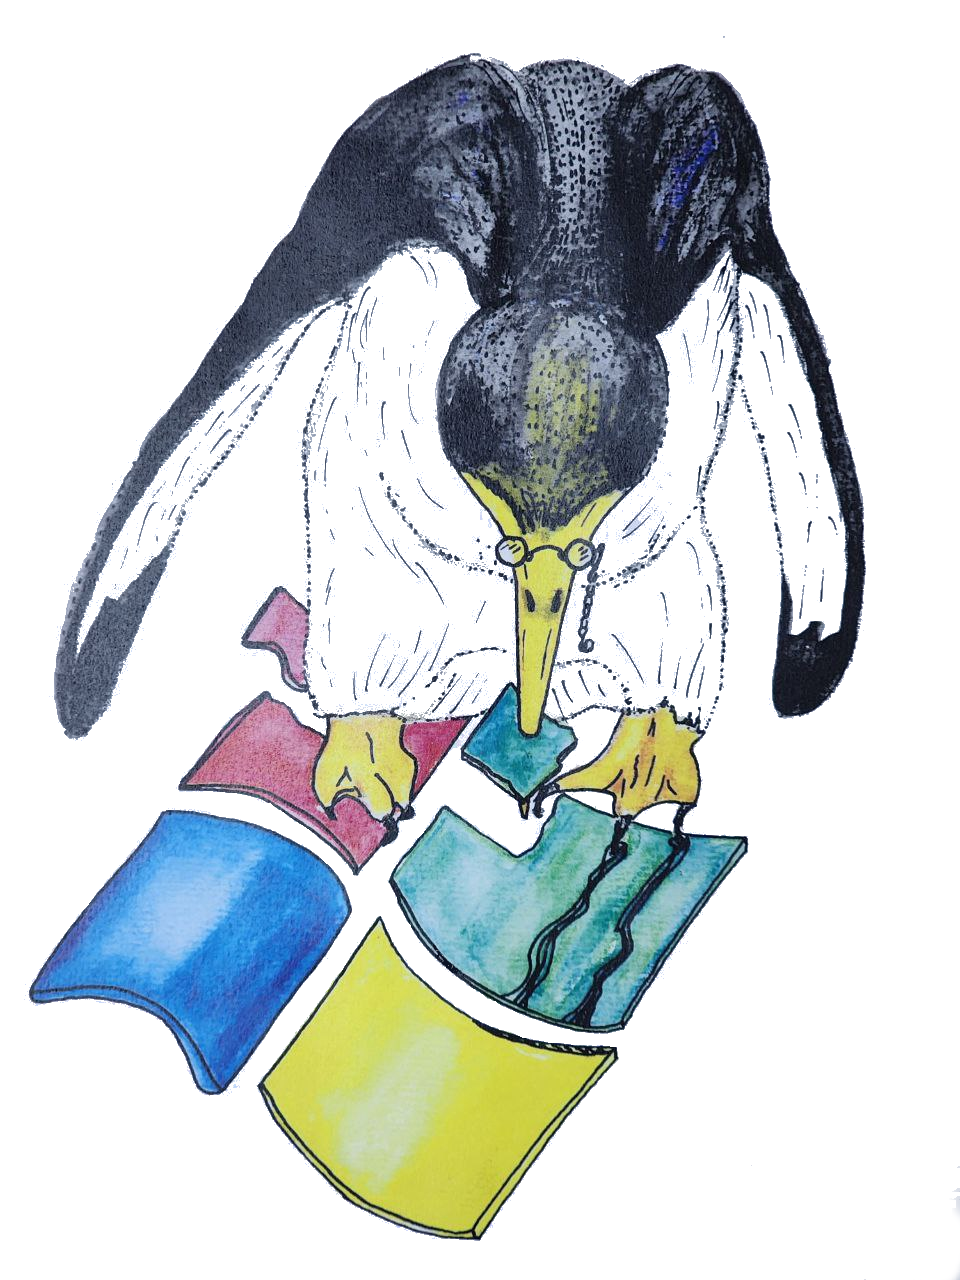
\epsfig{file=picts/gplt3/ping-win, width=4.5cm}
\end{center}

\vspace{-2cm}

\tableofcontents

\newpage
\section{Введение}
\begin{wrapfigure}[5]{t}{.3\textwidth}
  \vphantom{.}
  \vspace{-1.5cm}

  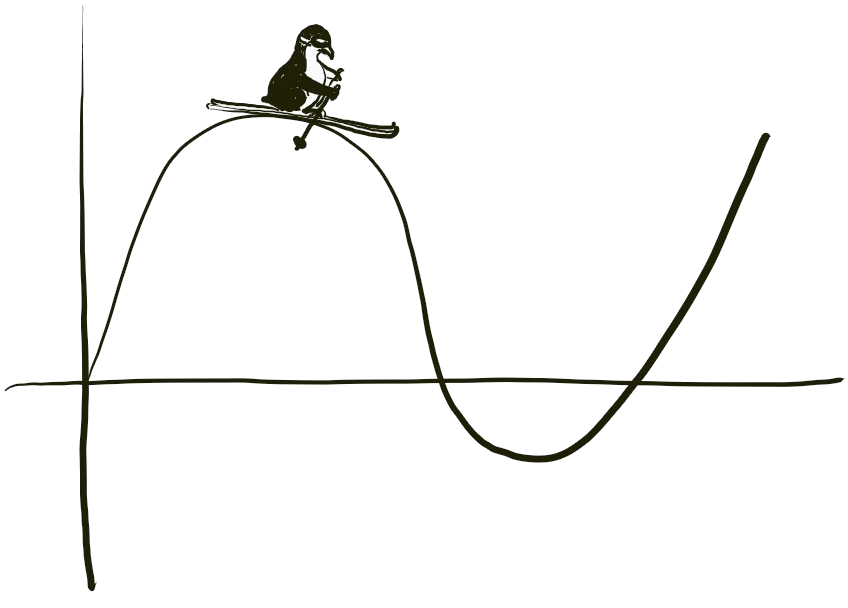
\epsfig{file=picts/gplt3/sin1, width=.27\textwidth}
\end{wrapfigure}
Первая версия утилиты \gplt{} появилась в начале нулевых годов, когда \gnuplot{} стал казаться автору слишком многословным.
На тот момент она называлась \verb'gnuplt' и была написана на \verb'bash'\footnote{Краткое описание той реликтовой версии утилиты можно найти в \cite{aiv:racs2007}.}.
С тех пор \gplt{} переписывалась несколько раз с нуля (при этом название скрипта становилось все короче),
сохраняя по возможности обратную совместимость с т.з. интерфейса.  

\def\gplt{{\tt gplt3}}

В настоящий момент утилита \gplt{} является скриптом на языке \python, разбирающим аргументы командной строки и формирующим команды для \gnuplot.
За счет коротких опций и различных умолчаний удается радикально уменьшить число нажатий клавиш. Кроме того, \gplt{}, как пылесос, собирает всю доступную информацию
(комментарии из заголовков файлов с данными и файлов.\RACS, \cite{aiwlib:SR:PP2018})
и старается на ее основе автоматически формировать подписи к осям, кривым и т.д.
Эта же информация позволяет давать столбцам имена и формировать из этих имен сложные математические выражения для построения.

Под графиками типографского качества понимаются графики с правильной шрифтовкой и зарамочным оформлением (как минимум подписями к осям и кривым)~---
т.е. графики, которые могут быть вставлены в печатную
работу, не вызывая замечаний со стороны самого требовательного корректора. Несмотря на бурное развитие вычислительной техники, подготовка таких графиков по-прежнему
остается кропотливой работой~--- утилита \gplt{} отчасти решает эту проблему.
Часть изменений в последней версии \gplt{} 2023 года как раз направлены на то, что бы упростить эту работу
еще больше за счет переиспользования введенных ранее команд. {\it<<Никакая информация не должна вводиться в компьютер дважды!>>}~--- в \gplt{} эта идея возведена в абсолют.
За один запуск \gplt{} способна сгенерировать целую серию рисунков с частично пересекающимися настройками.

Кроме рисования графиков на экране \gplt{} может генерировать картинки в форматах \png{} и \pdf.  При генерации \pdf{}  файлов используется терминал {\tt esplatex}
из \gnuplot, затем результаты автоматически прогоняются через \LaTeX{}, и у полученного файла обрезаются поля. С одной стороны, такой подход обеспечивает правильную
шрифтовку и позволяет использовать выражения \LaTeX{} в подписях к осям и кривым. С другой стороны, вставка одного \pdf{} файла вызывает
значительно меньше проблем, чем вставка пары файлов \verb'.tex' и \verb'.eps', генерируемых терминалом {\tt esplatex} в \gnuplot.

Для каждого сгенерированного рисунка \gplt{} создает одноименный  файл с расширением \verb'.gplt3', содержащий набор опций для генерации рисунка.
Файл является запускаемым (генерирует рисунок заново), что может быть полезно, если входные данные изменились.
Кроме того, файл может быть скопирован под другим именем, отредактирован вручную и применен для создания другого рисунка\footnote{Будьте внимательны ---
  имя рисунка явно прописано в {\tt .gplt3} файле, не забывайте его изменять при редактировании!}.

Опыт автора показывает, что самой лучшей оболочкой для обработки результатов численного моделирования (особенно если речь идет об HPC) является командная строка
с правильным набором утилит~--- например, \verb'yupiter' (\python3 с \verb'matlotlib') или \verb'matlab' оказываются в целом менее удобны, несмотря на свою <<заточенность>>
именно под такие задачи. Утилита   \gplt{} как раз является тем инструментом, который значительно расширяет возможности обычной командной строки,
позволяя быстро просматривать полученные результаты (в т.ч. без выкачивания их с удаленной машины при помощи терминала \verb'sixel')
и сразу строить рисунки типографского качества. 

Утилита \gplt{} распространяется под лицензией Апач 2.0, т.е. относится к ПО с открытым программным кодом, но может использоваться в коммерческих проектах
без согласования с автором.

\section{Установка  и настройка утилиты}
\begin{wrapfigure}{t}{.3\textwidth}
  \vphantom{.}
  \vspace{-3cm}

  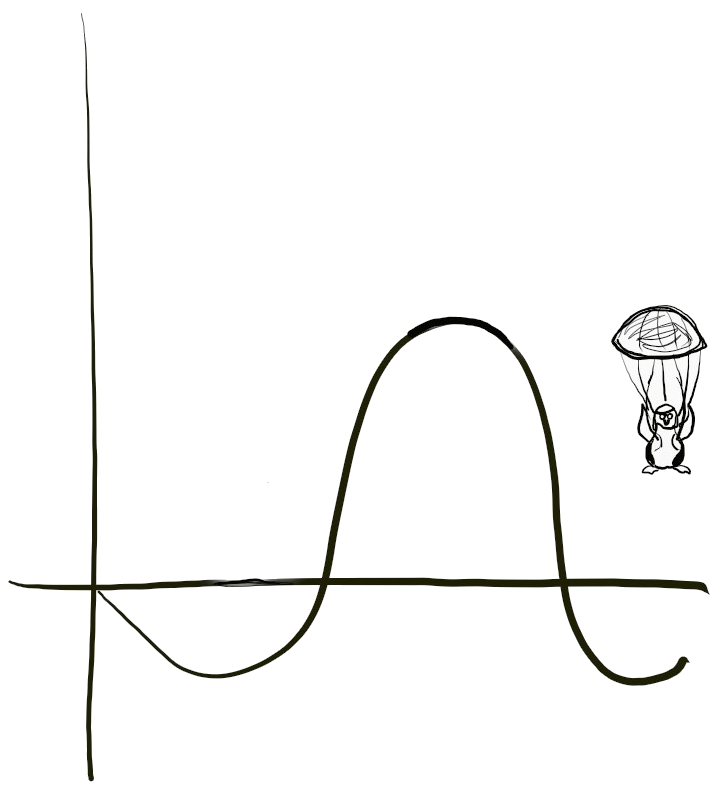
\epsfig{file=picts/gplt3/setup, width=.27\textwidth}
\end{wrapfigure}
Утилита \gplt{} написана для \verb'OS Linux', портирование под \verb'MS Windows' пока не проводилось. Скорее всего, утилита будет работать
под \verb'MS Windows' в среде \verb'WSL', но автор не имеет возможности полноценно проверить эту гипотезу.

Хотя утилита \gplt{} является частью библиотеки \verb'aiwlib' \cite{aiwlib:SR:PP2018,aiwlib:SV2018,aiwlib:git},
тем не менее, последняя версия выполнена в виде одного файла на языке \python, включающего в т.ч. достаточно подробную справку по утилите.
Такой подход несколько усложняет разработку (размер файла уже превысил 700 строк достаточно насыщенного кода), но значительно упрощает установку
неквалифицированными пользователями. Просто скопируйте \gplt{} в любую директорию из тропы поиска путей \verb'$PATH', например в \verb'~/bin':
\begin{verbatim}
$ mkdir ~/bin
$ export PATH=$PATH:~/bin
$ echo export PATH=\$PATH:~/bin >> ~/.bashrc
$ cd ~/bin && wget https://raw.githubusercontent.com/aivn/aiwlib/master/bin/gplt3 
$ chmod a+x gplt3
\end{verbatim}
Если у Вас уже есть директория \verb'~/bin/' и она присутствует в тропе поиска путей \verb'PATH', можно ограничиться последними двумя строчками.
Для обновления \gplt{} выполните
\begin{verbatim}
$ cd ~/bin && rm gplt3
$ wget https://raw.githubusercontent.com/aivn/aiwlib/master/bin/gplt3 
$ chmod a+x gplt3
\end{verbatim}

При установке библиотеки \verb'aiwlib' утилита \gplt{} будет установлена автоматически.

Для нормальной работы утилита \gplt{} требует как минимум установленного \gnuplot. Для генерации \pdf{} файлов требуются \verb'pdflatex', \verb'epstopdf'
и \verb'pdfcrop'. Для генерации \png{} файлов требуется утилита \verb'convert', обрезающая поля.

Все настройки \gplt{} хранятся в необязательном конфигурационном файле  \verb'~/.gplt3',
файл может быть создан командой
\begin{verbatim}
$ gplt3 -dump-config-file
\end{verbatim}
и отредактирован.
\newpage

\hrule
\begin{center}
\bf БУДЬТЕ ВНИМАТЕЛЬНЫ --- СТАРЫЙ ФАЙЛ С НАСТРОЙКАМИ,\\
ЕСЛИ ОН СУЩЕСТВУЕТ, БУДЕТ УНИЧТОЖЕН!
  \end{center}
\hrule
\phantom{.}

Файл содержит команды для запуска просмотрщиков \png{} и \pdf{} файлов, палитры для режима \verb'pm3d' и преамбулу \LaTeX{} документа для генерации \pdf{} файлов.

Кроме того, рекомендуется создать файл \verb'~/.gnuplot' следующего содержания:
\begin{verbatim}
set colors classic
set style data lines
set ticslevel 0
set grid front
\end{verbatim}

\section{Вызов справки}
Для вызова справки запустите \gplt{} без аргументов или с аргументом \verb'-h'. По опциям, отмеченным символом \verb'(*)',
есть более подробная справка, для ее получения запустите
\begin{wrapfigure}[3]{t}{.3\textwidth}
  
\epsfig{file=picts/gplt3/help, width=.27\textwidth}
\end{wrapfigure}
\begin{verbatim}
$ gplt3 -h <опция>
\end{verbatim}
например
\begin{verbatim}
$ gplt3 -h -fn
\end{verbatim}

Утилита \gplt{} позволяет выводить справку \gnuplot, для этого укажите интересующие Вас пункты после опции \verb'-h',
подпункты указываются через точку, например
\begin{verbatim}
$ gplt3 -h expression.functions
----------------------------  expression.functions  ----------------------------
 Arguments to math functions in `gnuplot` can be integer, real, or complex
 unless otherwise noted.  Functions that accept or return angles (e.g. sin(x))
...
\end{verbatim}
Если Вы используете \gnuplot, возможно, \gplt{} имеет смысл установить только для быстрого доступа к справке \gnuplot{} из командной строки.

Справка по многим опциям \gplt{} выводит справку по соответствующим опциям \gnuplot, например
\begin{verbatim}
$ gplt3 -h -sk
------------------------------------  -sk  -------------------------------------
 The `set key` command enables a key (or legend) containing a title and a
 sample (line, point, box) for each plot in the graph. The key may be turned off
...
\end{verbatim}

Интересующие опции и пункты справки \gnuplot{} (в т.ч. с подпунктами) могут указываться после опции \verb'-h' через пробел в любом порядке и количестве
(если листать вверх длинный вывод утомительно, используйте перенаправление \verb'| less'), важно только чтобы опция \verb'-h' шла первой.
В этом руководстве не очень много примеров~--- Вы всегда можете проверить интересующую Вас комбинацию опций самостоятельно, это быстро и безопасно. 
\pagebreak

\section{Общие замечания}\label{main:sec}
Утилита \gplt{} разбирает опции командной строки и формирует на их основе последовательность команд для \gnuplot. Если Вы хотите посмотреть,
какая именно последовательность команд будет отправлена в \gnuplot, добавьте опцию \verb'-debug' в (почти!) любое место~--- вместо \gnuplot{}
сформированная последовательность команд будет направлена на стандартный вывод:\footnote{Часть работы
  (чтение стандартного ввода, чтение заголовков файлов и т.д.) при этом будет все равно скрыта.}
\begin{wrapfigure}[1]{t}{.3\textwidth}
  \vphantom{.}
  \vspace{-1.3cm}

  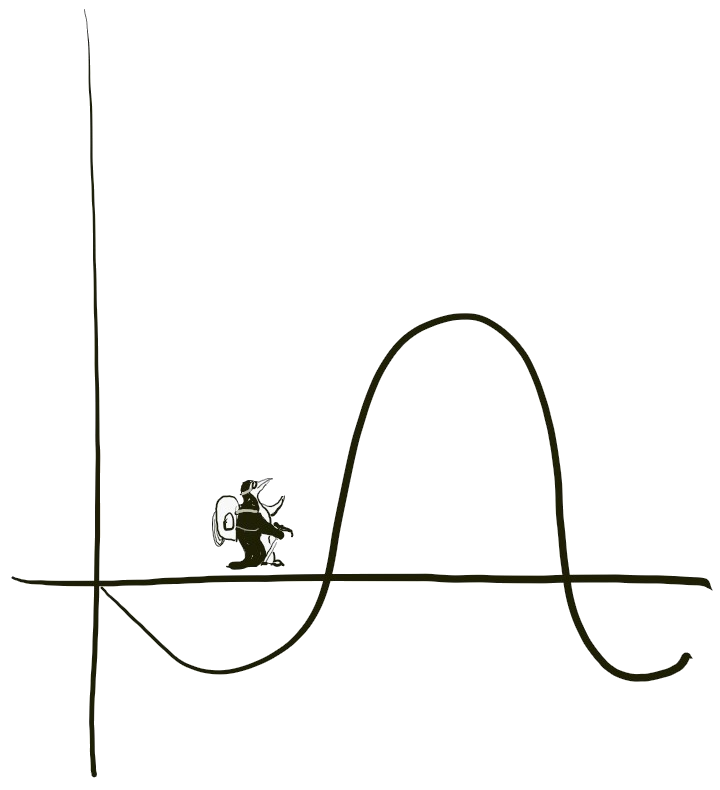
\epsfig{file=picts/gplt3/sin2, width=.27\textwidth}
\end{wrapfigure}
\begin{verbatim}
$ gplt3 -fn x**2 -debug
#>>> -fn 'x**2'
set xlabel 'x'
set ylabel 'x**2'
plot x**2 notitle   
pause -1
\end{verbatim}

\vspace{5mm}

Синтаксис аргументов командной строки \gplt{} тривиален и может быть сформулирован в трех пунктах:
\begin{enumerate}
\item опции командной строки начинаются с одинарного знака <<минус>>;
\item некоторые опции командной строки имеют один (и только один) аргумент, если аргумент пуст, то все равно надо указывать пустые кавычки \verb|''| или \verb|""|;
\item все, что не является опцией или аргументом опции, трактуется как имя файла с данными для отрисовки.
\end{enumerate}
\begin{verbatim}
$ gplt3 -nk          ...         -fn 'sin(x)'     ...     result.dat
        ^ опция без аргументов   ^ опция и ее аргумент    ^ файл с данными
\end{verbatim}
Порядок следования опций и файлов с данными не фиксирован, но {\bf может} иметь значение.  Некоторые опции имеют синонимы, например \verb'-U' и \verb'-u'
(задает кривые из файла для отрисовки) или \verb'-w' и \verb'-ds' (глобально задает стиль отрисовки).

Одни и те же файлы с данными, включая стандартный ввод который обозначается как~\verb'-' (знак <<минус>>) или \verb'-std', можно указывать многократно в любом порядке,
но заголовок каждого файла будет прочитан только один раз, реальное чтение данных со стандратного ввода тоже будет проводится однократно.
Каждый файл с данными {\bf при первом упоминании} добавляется в общий список файлов. 
К уже указанным файлам можно обращаться по номерам (в квадратных скобках) в синтакисе \python, например \verb'[-1]'~--- последний из файлов списка,
\verb'[0] [-1]'~--- первый и последний из файлов списка (список при этом {\bf не} меняется), \verb'[:]'~--- весь список файлов.
При обращение к файлам по номерам можно использовать @-атрибуты (см. следующий раздел \ref{dog:attr:sec}). 

Поддерживается работа с обычными \verb'.dat'-файлами (данные в несколько колонок, резделители пробелы или знак табуляции) и \verb'.csv'-файлами
(разделители \verb';' или \verb','), файлы могут быть сжаты при помощи \verb'gzip' (дополнительное расширение \verb'.gz').
Кроме того, в качестве источника данных можно использовать фильтры~--- \verb'bash' команды пишушщие данные на стандартный вывод.
Для задания фильтра надо указать вначале \verb'!', например \verb|gplt3 '!echo  "1 2\n3 4"'|.

%\newpage

По семантике все опции можно разделить на следующие группы.
\begin{enumerate}
\item Простые опции, включающие/выключающие какой-то режим (например \verb'-3d', \verb'-2d')
  и/или добавляющие команду для \gnuplot{} (например, \verb'-sk <keyopt>' настраивает легенду, передавая в \gnuplot{} команду \verb'set key <keyopt>').
  Самыми яркими представителями являются \verb'-s <command>' (просто передает в \gnuplot{} строку \verb'set <command>'),
  \verb'-us <command>' (передает \verb'unset <command>') и совсем брутальная \verb'-raw <command>', передающая \verb'<command>'~---
  эти опции введены для каких-то экзотических случаев и не рекомендуются для использования. 
\item Опции (с аргументами) явно устанавливающие подписи к осям~--- \verb'-lbx', \verb'-lby', \verb'-lbz', \verb'-lbcb', \verb'-lbx2', \verb'-lby2'
  и титул рисунка \verb'-ttl'. Аргументы этих опций обрабатываются специальным образом с учетом метаинформации (из заголовков файлов с данными и \verb'.RACS') и
  могут быть преобразованы в \LaTeX{}.
\item Опции, задающие, что именно рисовать и откуда:
  \begin{enumerate}
  \item \verb'-fn <function>' --- добавляет аналитическую функцию;
  \item \verb|-U '<expr1> <expr2> ...'| --- необязательная опция, задающая, какие именно зависимости надо рисовать из файлов с данными, действует на {\bf все} файлы,
    следующие после себя, пока не встретится другая опция \verb'-U';
  \item собственно, файлы с данными. 
  \end{enumerate}
\item Специальные опции, определяющие логику работы \gplt{} и структурирующие последовательность аргументов в командной строке:
  \begin{enumerate}
  \item \verb'-to <filename>' --- терминирующая опция, отрисовывающая все, что было накоплено с предыдущей опции \verb'-to', имя файла может иметь расширение \png, \pdf{}
    или быть пустым (\verb|""|, отрисовка на экран). Если последняя опция \verb'-to' не указана, то она все равно будет вызвана с отрисовкой на экран.
  \item \verb'-o <origin>' --- <<лайт>>-версия опции \verb'-to' внутри режима \verb'multiplot' (несколько графиков на одном рисунке). Включает режим
    \verb'multiplot', опция \verb'-to', соответственно, создает рисунок со всеми графиками и выключает режим \verb'multiplot'.
  \item\verb'-i <filename>' --- модифицирует последовательность аргументов командной строки, вставляя на свое место опции из файла \verb'<filename>',
    повторная вставка того же файла блокируется для защиты от зацикливания.
  \end{enumerate}
\end{enumerate}
Кроме того, в \gplt{} есть циклы и макросы (см. раздел \ref{clif:sec}), но они совершенно не обязательны к использованию, имеют свой синтаксис, и пока что
о них можно не думать.
\newpage

\section{<<Собачьи>> @-атрибуты}\label{dog:attr:sec}
\begin{wrapfigure}[5]{t}{.3\textwidth}
  \vphantom{.}
  \vspace{-2.5cm}

  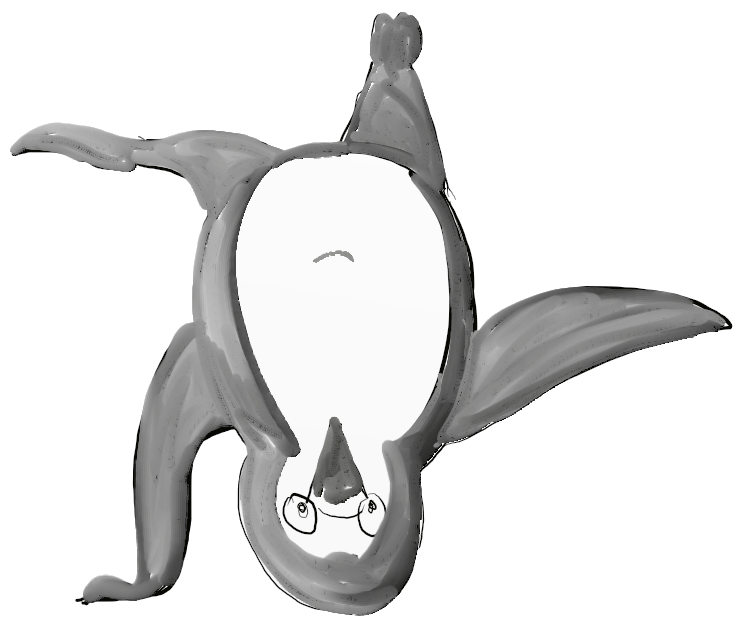
\epsfig{file=picts/gplt3/acrobat, width=.27\textwidth}
\end{wrapfigure}
В какой-то момент во время эволюции и эксплуатации \verb'gplt' возникла острая необходимость для быстрого, точечного задания некоторых ключевых
параметров кривых~--- толщины, цвета и т.д. Как иногда бывает, сделанный <<на коленке>> вариант
оказался настолько удобным, что вытеснил остальные варианты. 

%\enlargethispage{9mm}
Что делать, если мы договорились, что опция не может иметь больше одного аргумента, но именно этот аргумент мы иногда хотим дополнить какими-то необязательными атрибутами,
причем сделать это как можно лаконичнее?
Разумеется, расширить синтаксис. Для расширения синтаксиса в данном случае используется символ <<собака>> \verb'@', за которым через запятую дописываются те самые
дополнительные атрибуты. Например,
\begin{verbatim}
$ gplt -fn x**2@5,blue,dots
\end{verbatim}
нарисует кривую $x^2$ голубыми точками размером в 5px.

Существует два типа @-атрибутов~--- для подписей к осям «цвет», «смещение» и «поворот»; для кривых (аналитических функций,
имен файлов и аргументов опции \verb'-U') можно задавать толщину, цвет, стиль, оси отображения и подпись на легенде.
Все эти параметры так или иначе устанавливаются \gplt{} по умолчанию, @-опции нужны для явного и лаконичного исправления ситуации, если что-то пошло не совсем так. 

Важной особенностью @-атрибутов является их наследуемость, то есть, если какой-то из атрибутов не задан, то он считается задаваемым по умолчанию
обычными алгоритмами \gplt, но ситуация может быть уточнена/исправлена в дальнейшем.
Как уже отмечалось выше, опция \verb'-U' задает одну или несколько кривых для отрисовки из следующих за ней файлов. При выводе на экран по умолчанию
все кривые рисуются линиями толщиной 1px, при выводе в файл 3px (на бумаге и/или в презентации линии кажутся тоньше).
Если указать \verb'-U x**2@5', то из последующих файлов будут строиться кривые $x^2$ толщиной 5px, но если какой-то из файлов задать как
\verb'filename.dat@2', то из него кривая $x^2$ будет построена с толщиной 2px~---. Поскольку толщина линии для файла \verb'filename.dat' задается позже, чем в \verb'-U',
то она имеет более высокий приоритет для данного файла, но не действует на остальные файлы. 

<<Собачьи>> @-атрибуты указываются после символа @ через запятую в произвольном порядке (единственным исключением является задание подписи к кривой на легенде,
она всегда указывается последней и начинается со знака \verb'='). 

Для подписей к осям доступны следующие @-атрибуты:
\begin{itemize}
\item смещение подписи/титула --- число;
\item цвет подписи/титула --- имя цвета;
\item поворот --- \verb'r<целое-число>'.
\end{itemize}
Например, \verb'-lbx runtime@1.5,4,r90,red' установит по оси $x$ подпись \verb'runtime' красного цвета, повернутую на $90^\circ$ со смещением в 1.5, 4.
Как уже отмечалось выше, порядок следования атрибутов произвольный, \verb'-lbx runtime@1.5,red,r90,4' даст точно такой же эффект (но 1.5 должно идти раньше 4),
указывать можно не все атрибуты, а только необходимые. 
Компоненты смещения задаются в единицах характерного размера символа, можно указывать не все компоненты, а первые сколько-то необходимых (скажем только по $x$).
Важной особенностью является возможность указания только @-атрибутов без текста подписи, например \verb'-lbx @1.5,red,r90,4' задаcт смещение, цвет и поворот
подписи, но текст подписи будет определяться автоматически на основе выражений для отрисовки.

Ну и наконец, \verb'-lbx ""' убирает подпись по оси $x$, \verb'-lbx <text>' устаналивает текст метки с атрибутами по умолчанию, 
\verb'-lbx @' возвращает полностью автоматический режим выбора текста подписи с атрибутами по умолчанию\footnote{Смещения нет, поворота нет, цвет черный.}.

Для выражений в \verb'-fn', \verb'-U' и для имен файлов доступны следующие @-атрибуты:
\begin{itemize}
\item толщина линии --- целое положительное число (по умолчанию 1 для вывода на экран и 3 для отрисовки в файл);
\item цвет линии --- имя цвета (по умолчанию выбирается \gnuplot-ом, зависит от номера кривой на графике);
\item оси отображения --- \verb'x1y1', \verb'x1y2', \verb'x2y1', \verb'x2y2' (по умолчанию \verb'x1y1');
\item подпись к кривой на легенде --- начинается с \verb'=', должна идти последней (по умолчанию задается \gplt{} на основе информации о том, что именно рисуется);
\item стиль отрисовки --- все, что не относится к предыдущим пунктам. Вариантов \gnuplot{} предоставляет довольно много, например \verb'l' (\verb'lines'),
  \verb'p' (\verb'points') и т.д., см.
\begin{verbatim}
$ gplt3 -h style
...
Subtopics available for style:
    arrows            boxerrorbars      boxes             boxplot
    boxxyerror        candlesticks      circles           dots
    ellipses          errorbars         errorlines        filledcurves
    fillsteps         financebars       fsteps            histeps
    histograms        image             impulses          isosurface
    labels            lines             linespoints       lp
    points            polygons          rgbalpha          rgbimage
    steps             vectors           xerrorbars        xerrorlines
    xyerrorbars       xyerrorlines      yerrorbars        yerrorlines
    zerrorfill
\end{verbatim}
\end{itemize}

\section{Заголовки файлов с данными и другие источники метаинформации}\label{metainfo:sec}
\begin{wrapfigure}[5]{t}{.3\textwidth}
  \vphantom{.}
  \vspace{-1.2cm}

  
\epsfig{file=picts/gplt3/table, width=.27\textwidth}
\end{wrapfigure}
Мы уже несколько раз упоминали заголовки \verb'.dat'-файлов, пора остановиться на них поподробнее.

С точки зрения \gnuplot, все строчки в \verb'.dat'-файле, начинающиеся с символа \verb'#', являются комментариями. С точки зрения \gplt{},
имеют значение строки, начинающиеся с \verb'#:'
\begin{verbatim}
# пример заголовка для gplt3
#: R = 8.31   # универсальная газовая постоянная
#: rho_H2O, C_H2O = 1e3, 4200  # плотность и теплоемкость воды
#: rho_Fe = 7800;  C_Fe = 460  # плотность и теплоемкость железа
#: t rho T mu
#: mu.tex = '\\omega_1'  # задаем LaTeX представление для mu
0. 12  1e-3  14
...
\end{verbatim}
Здесь представлено задание пяти параметров ($R$, $\rho_{\rm H2O}$, $C_{\rm H2O}$, $\rho_{\rm Fe}$, $C_{\rm Fe}$) и задание имен для четырех столбцов файла с данными.
Чтение заголовка прекращается после первой же строки с данными (числами), дальше \gplt{} заглядывать не будет. В задаваемых через опцию \verb'-U'
выражениях можно будет обращаться по именам к столбцам, при конвертации в формат \gnuplot{} для отрисовки они будут выглядеть как \verb'($1)', \verb'($2)' и т.д.
Порядок следования при задании имен столбцов и параметров не имеет значения~--- можно указывать имена столбцов в начале, а параметры в конце, или задавать имена столбцов
где-то между строчками с заданием параметров. Строки с заданным параметром (такими считаются строки, начинающиеся с \verb'#:' и содержащие знак \verb'=')
обрабатываются функцией
\begin{verbatim}
exec(src_line, {'__builtins__': None}, dst_scope)
\end{verbatim}
и попадают в словарь \verb'dst_scope'. Глобальное пространство имен вида \verb|{'__builtins__': None}| обеспечивает безопасность, отключая все
встроенные функции \python{}, т.е. код
\begin{verbatim}
#: import os; os.system('rm -rf ~/')
\end{verbatim}
не будет выполнен\footnote{<<Можно придумать защиту от дурака, но только от неизобретательного>> {\it Закон Нейсдра.}}. 

В примере в последней строке заголовка задается \LaTeX{} версия для имени столбца \verb'mu', на экране и \png{} рисунках эта переменная
будет выглядеть как \verb'mu', на рисунках \pdf{} как $\omega_1$ (такое различие в обозначениях не кажется хорошей идеей, это просто пример).
Важно, что \verb|'\\omega_1'| это именно строка (в кавычках), и что там стоит именно два бэкслэша \verb'\\' (первый бэкслэш экранирует второй).
Аналогичный результат можно получить, написав \verb|r'\omega_1'|. Обрамление в \verb|r'$\omega_1$'| здесь не требуется и, напротив, будет являться
ошибочным~--- \gplt{} расставляет \$ сам.
%Особенно важно то, что задание \verb'#: mu.tex = ...' идет {\bf после}
%задания имен столбцов~--- до этого момента имя \verb'mu' не определено как имя столбца.
В старых версиях \verb'gplt' необходимо было указывать \LaTeX{} версии имен столбцов после того, как имена столбцов заданы.
В \gplt{} этот порядок уже не имеет значения, строки с заданием имен столбцов в любом случае обрабатываются в первую очередь.
Не спешите задавать \LaTeX{} версии имен столбцов~--- \gplt{} генерирует их самостоятельно в большинстве простых случаев.

Число имен в строке, задающей имена столбцов, не обязательно должно совпадать с числом столбцов с данными~--- если имен будет меньше, Вы не сможете обратиться к
последним столбцам (на самом деле сможете, но по-другому), если имен будет больше, при обращении к несуществующему столбцу \gnuplot{} выдаст ошибку.
Допустимо задание нескольких вариантов имен столбцов в нескольких разных строках, это приведет к тому, что у столбцов будет по несколько имен.
Если какое-то имя будет продублировано, актуальным станет последняя версия имени:
\begin{verbatim}
#: A B C
#: C D E
\end{verbatim}
В этом странном примере к первому столбцу можно обращаться по именам \verb'A' и \verb'C', ко второму~--- \verb'B' и \verb'D', к третьему только \verb'E'.
При построении этого файла по умолчанию (без опции \verb'-U') актуальным с точки зрения подписей к осям будет последний комплект имен столбцов. 

По умолчанию с точки зрения \gplt, первые три столбца имеют имена \verb'x', \verb'y', \verb'z', кроме того, первые 255 столбцов имеют имена \verb'C1' ... \verb'C255',
имя \verb'C0' обозначает номер строки, и на сегодняшний день это единственный способ обратиться к номеру строки. 

В \gplt{} можно задавать столбцы как компоненты вектора, например,
\begin{verbatim}
#: t E.x E.y E.z P 
\end{verbatim}
или
\begin{verbatim}
#: t E[0] E[1] E[2] P 
\end{verbatim}
или даже
\begin{verbatim}
#: t E[] E[] E[] P 
\end{verbatim}
Здесь \verb't' и \verb'P' --- обычные скалярные параметры, \verb'E' - векторный параметр.
В первом случае имена у компонент вектора могут быть любыми идентификаторами, обращаться к компонентам в выражении можно
по именам (через точку) или по номерам в том порядке, в котором они были указаны, например, \verb'E[0]' вместо \verb'E.x' и т.д.
Во втором и третьем случаях обращаться к компонентам в выражении можно только по номерам.
Во втором случае последовательность компонент
 вектора может быть любой, но важно, чтобы номера компонент были от $0$ до $D-1$, где $D$~--- размерность вектора. В третьем случае
 номера компонентам вектора будут розданы автоматически, начиная с нуля.
Во всех случаях компоненты могут идти вперемешку с обычными скалярными параметрами, три примера:
\begin{verbatim}
#: t E.x P E.y E.z  
#: t E[0] P E[1] E[2]
#: t E[] P E[] E[]  
\end{verbatim}
хотя это и будет выглядеть странно.
В выражениях, кроме обращения к компонентам вектора, можно брать модуль вектора как \verb'E.abs()', \verb'abs(E)',  \verb'fabs(E)' или даже  \verb'|%E%|',
скалярно перемножать вектора при помощи~\verb'*',
умножать вектор на скаляр и скаляр на вектор при помощи~\verb'*', складывать и вычитать вектора, а также вычислять векторное произведение при помощи \verb'%'
(определено только для 2D и 3D векторов).

Неоднократно упоминавшиеся файлы \verb'.RACS' содержат словарь с параметрами расчета в формате \verb'pickle'.
Эти файлы создаются \verb'RACS' (системой контроля результатов и алгоритмов,~\cite{aiwlib:SR:PP2018}).
Каждый раз, обрабатывая файл с данными, \gplt{} ищет файл \verb'.RACS' вверх по дереву директорий, начиная от директории, содержащей файл с данными,
и вплоть до корня файловой системы. Параметры из файла \verb'.RACS' могут быть использованы в различных выражениях, включая подписи к кривым на легенде и
заголовок рисунка.

При работе с \verb'.csv'-файлами опционально заголовок может занимать первую строчку и содержать только имена столбцов. Никакой символ комментирования не требуется,
имена столбцов идут через тот же разделитель что и весь остальной файл~--- разделитель \verb';' или \verb',', для всего файла раздилетль должен быть один и тот же.
Первая строка трактуется как заголовок если первый элемент первой строки не может быть приведен к \verb'float'.
Векторные имена столбцов для \verb'.csv' не поддерживаются.

\section{Ввод и преобразование выражений, автоматическая генерация подписей}
\begin{wrapfigure}[8]{t}{.3\textwidth}
  \vphantom{.}
  \vspace{-1cm}

  
\epsfig{file=picts/gplt3/quest, width=.27\textwidth}
\end{wrapfigure}
Это, наверное, самый важный и сложный для понимания раздел руководства, но в тоже время самый интересный. 

Выражением здесь мы будем называть некоторое алгебраическое выражение, например $a x$, $2$, $A + B\sin^2\omega t$ и т.д. Выражение всегда вводится
в синтаксисе \python{} {\bf без} пробелов, например, \verb'a*x', \verb'2', \verb'A+B*sin(omega*t)**2' и т.д.
При задании аналитической функции через {\tt -fn} и в подписях к осям/титулу пробелы не страшны, если они
  заэкранированы от {\tt bash}, но для опции {\tt -U} пробелы являются разделителями аргумента. 

  Сразу отметим, что \gplt{} несколько расширяет синтаксис \python{}, вводя дополнительные скобки (в обычном, алгебарическом смысле) как
\verb'(%...%)', \verb'[%...%]', \verb'', \verb'<%...%>', \verb'' и \verb'|%...%|', где под \verb'...' понимается законченный фрагмент выражения.
Забранный в скобки фрагмент выражения, как обычно, может являться частью большего выражения, но при отображении в текст его скобки будут выводиться всегда, например,
\verb'a*[%(%b%)+(c*d)%]' даст в \LaTeX{}
$a[(b)+c\,d]$~--- обратите внимание, что здесь \verb'(c*d)' выводится без скобок, поскольку они не требуются
с т.з. приоритета операций. При выводе в \LaTeX{} к скобкам добавляются \verb'\left' и \verb'\right'. Скобки \verb'|%...%|' трактуются как модуль,
в том числе и при конвертации выражения в \gnuplot{}, а функции \verb'abs(...)' и \verb'fabs(...)' воспринимаются как \verb'|%...%|'.

Доступны все операции \python{}, операция \verb'//' трактуется как обычное деление, но при выводе в \LaTeX{} конвертируется во \verb'\frac'.
Операция \verb'^' воспринимается {\bf не} как степень, а как побитовый \verb'xor'.

Операция \verb'(...)' перегружена и может применяться в двух случаях:
\begin{enumerate}
\item для задания аргументов функции отрисовки из файла (по умолчанию строится зависимость от первого или первых двух столбцов);
\item для замены переменных в выражении на другие выражения, что иногда требуется при работе с макросами (см. раздел \ref{clif:sec}),
  например, \verb'f:=sin(x*a) ... {f}(a=y)' даст в итоге функцию \verb'sin(x*y)'
\end{enumerate}
Оба этих режима могут действовать одновременно:
\begin{verbatim}
(sin(x*a))(C3,a=y) <==> (sin(x*y))(C3)
\end{verbatim}
Большое значение имеет, для какого фрагмента выражения применяется операция \verb'(...)', например,
\begin{verbatim}
 cos(x*a)+sin(x*a)(a=y)  <==> cos(x*a)+sin(x*y)
(cos(x*a)+sin(x*a))(a=y) <==> cos(x*y)+sin(x*y)
\end{verbatim}

Преобразование выражений действует по одному и тому же алгоритму (с небольшими нюансами)~--- после обработки расширенного синтаксиса скобок выражение преобразуется в AST
(абстрактное синтаксическое дерево), затем полученная структура может быть преобразована к одному из трех форматов: \gnuplot{} (для генерации
строки \verb'plot ...'), текстовому (для отображения на экране или в \png{} файле) или \LaTeX{} (для генерации \pdf).
AST состоит из экземпляров классов, реализующих операции \python, по одному классу на каждую операцию (\verb'AddOp' для \verb'+', \verb'MulOp' для \verb'*'
и т.д., \cite{aiv:symbalg:MM2015}),
классы определены непосредственно в теле утилиты \gplt. Разбор выражения \verb'expr' производится при помощи функции
\begin{verbatim}
eval(expr, {'__builtins__': None, ... globalscope...}, {...localscope...})
\end{verbatim}
из соображений безопасности все встроенные функции \python{} при этом отключены. В глобальном контексте \verb'globalscope' размещаются математические функции:
\begin{verbatim}
  abs      fabs   acos acosh airy  asin asinh atan  atanh atan2 ceil   cos  
  cosh     ch     ctg  cth   erf   exp  floor gamma ifch  int   inverf invnorm 
  lambertw lgamma log  ln    log10 lg   min   max   norm  sgn   sin    sinh    
  sh       sqrt   tan  tg    tanh  th   !     !!
\end{verbatim}
Функция \verb'ifch(<expr1>,<cond1>,<expr2>[,<cond2>,<expr3>,...])'  трактуется как цепочка
\verb'<expr1> if <cond1> else <expr2> if <cond2> else <expr3> ...' Функции \verb'min' и \verb'max' могут принимать произвольное число аргументов. Факториалы имеют такой же приоритет как возведение в степень \verb'**'.
Подробнее см. \verb'$ gplt3 -h expressions.functions plot'.
Все самое интересное связано с локальным контекстом \verb'localscope'.

AST для выражения это ациклический направленный граф, листьями AST являются числа или переменные. 
Есть два разных режима преобразования выражений (зачастую одного и того же выражения):
\begin{itemize}
\item преобразование выражения в формат \gnuplot{} для фунцкии \verb'plot',  в этом случае все переменные должны быть заменены на числа
  или на номера столбов \verb'dat'-файла  в виде \verb'($1)', \verb'($2)' и т.д.;
\item преобразование выражения для подписей в форматы \verb'txt' или \LaTeX{}, в этом случае, напротив, вместо чисел желательно использовать имена переменных,
 при выводе в \LaTeX{} нужно, по возможности, дать именам переменных их \LaTeX-версии, например, заменить \verb'omega0' на \verb'\omega_0'.
\end{itemize}
%Кроме формата вывода, эти режимы отличаются содержимым \verb'localscope', причем это отличие принципиальное~--- если в первом режиме
%использование неизвестной переменной должно приводить к ошибке, то во втором режиме использование произвольного набора имен вполне допустимо.
%В первом режиме \verb'localscope' это словарь, содержащий переменные, ассоциированные с параметрами расчета, полученными из файла~\verb'.RACS',
%заголовка \verb'.dat'-файла и номерами столбцов \verb'.dat'-файла. Во втором режиме все переменные, даже те, которые ассоциированы с параметрами расчета (числа),
%отображаются под своими именами для наглядности. Кроме того,
Во всех случаях \verb'localscope' допускает обращение к переменным с произвольными именами, но при преобразовании выражения
для отрисовки в \gnuplot{} все имена должны быть разрешены через переменные, ассоциированные с параметрами расчета, полученными из файла~\verb'.RACS',
заголовка \verb'.dat'-файла и номерами столбцов \verb'.dat'-файла ии переменными $x$, $y$ при отрисовке функций.
Под разрешением переменных понимается использование операции \verb'()' для замены переменных на выражения/другие переменные. 
%При выводе в \LaTeX{} для наглядности рациональные числа будут выводиться в виде дробей,
%если числитель и знаменатель по модулю не превышают девяти, например, \verb'0.333333333333333' будет заменено на $\frac13$.

Можно сформулировать следующие правила относительно переменных при задании выражений для {\bf отрисовки}.
\begin{enumerate}
\item При задании обычной функции (опция \verb'-fn') аргументами функции могут являться переменные $x$ в \verb'-2d' случае или $x, y$ в \verb'-3d' случае.
\item При задании параметрической функции (опция \verb'-fn', где-то перед которой стоит опция \verb'-par')
  аргументами функции могут являться переменные $t$ в \verb'-2d' случае или $u, v$ в \verb'-3d' случае. Во всех случаях параметрическая функция задается как
  кортеж выражений (выражения следуют через запятую), число элементов кортежа должно отвечать размерности графика:
\begin{verbatim}
$ gplt3 -par -fn 'sin(t),cos(t)'                            # окружность
$ gplt3 -par -3d -fn 'sin(u)*sin(v),cos(u)*sin(v),cos(v)'   # сфера
\end{verbatim}
\item При задании кривых для отрисовки из файла (опция \verb'-U', несколько кривых должны быть отделены пробелом, и в этом случае обязательны кавычки, поскольку с т.з.
  шелл это должен быть один аргумент опции) в качестве аргументов можно использовать любые имена столбцов, в том числе имена столбцов по умолчанию.
\begin{verbatim}
$ echo "#: a, b = 1, 2.5" > test1.dat 
$ echo "#: A B C" >> test1.dat 
$ python3 -c 'for i in range(100): print(i, i**2, i**3)' >> test1.dat
$ gplt3 test1.dat             # кривая B(A), кавычки не обязательны.
$ gplt3 -U 'a*B C' test1.dat  # кривые (2*B)(A) и C(A), здесь кавычки обязательны!
\end{verbatim}
\item По умолчанию при отрисовке из файла по осям $x$ (и $y$ в \verb'-3d' случае) откладываются значения из первого (и второго в \verb'-3d' случае) столбцов.
  Аргументы кривой можно изменить, указав новые аргументы в скобках, как для обычной функции, лучше взять выражение в скобки:
\begin{verbatim}
$ gplt3 -U 'С C(B) (A+2*C)(B**2)' test1.dat  # кривые C(A) и т.д.
\end{verbatim}
\item Можно задавать кривую в \verb'-U' как кортеж в порядке возрастания осей, т.е. вместо \verb|-U 'C(B)'| писать \verb'-U B,C'. При использовании
  стилей, требующих много компонентов (например \verb'errorbars'), это единственный способ указать все необходимые компоненты. Кортеж транслируется в выражение
  для \gnuplot{} через \verb':' (попробуйте добавить опцию \verb'-debug').
\item Все остальные символы в выражениях должны быть параметрами из заголовков \verb'dat'-файла или \verb'.RACS'. 
При задании функции доступны все параметры из использованных ранее на этом графике \verb'dat'-файлов и связанных с ними файлов \verb'.RACS'.
\begin{verbatim}
$ gplt3 -fn a+b*x  test.dat  # ошибка, a и b не определены
$ gplt3 test.dat -fn a+b*x   # кривые B(A) и 1+2.5*x, фактически 1+2.5*A
$ gplt3 test.dat -to '' -fn a+b*x  # ошибка, после -to уже нет a и b
\end{verbatim}
Если есть несколько файлов с перекрывающимися параметрами, актуальными являются значения параметров из последнего файла
\begin{verbatim}
$ echo "#: b, c = -3, 4" > test2.dat 
...
$ gplt3 test1.dat test2.dat -fn a+b*x+c*x**2  # функция 1-3*x+4*x**2
\end{verbatim}
\end{enumerate}

При явном задании подписей действуют другие правила.
Мы будем говорить о правилах преобразования некоторого выражения \verb'epxr', встречающегося в аргументах опций
\verb'-lbx', \verb'-lby', ... (подписи к осям),  \verb'-ttl' (титул графика) и @-атрибутах \verb'-U' и \verb'-fn' после знака \verb'='
(явное задание подписей кривых на легенде).   
\begin{enumerate}
\item Как и в предыдущем случае, выражение должно быть введено в расширенном (за счет скобок) синтаксисе языка \python,
  затем оно будет преобразовано к AST при помощи \verb'eval'. Если такие преобразования не нужны, то в конце выражения
  нужно поставить \verb'!'~--- тогда оно останется без изменений при выводе на экран/в \png, при построении \pdf{} в выражении
  будут заэкранированы специальные символы \LaTeX{}\footnote{Идеальным было бы применение {\tt $\backslash$verb}, но через терминал {\tt epslatex}
    это не работает в сложных случаях}.  
  Если никакие преобразования не нужны, в конце выражения нужно поставить \verb'!!'. Если Вам нужен \verb'!' в конце выражения сам по себе,
  добавьте после него пробел~--- в любом случае здесь с т.з. шелл будут нужны кавычки.
\item При задании подписей функций и кривых из файлов действуют те же правила относительно параметров, что и при создании выражений для отрисовки~---
  кривая из файла <<видит>> все параметры из заголовка файла и связанного (лежащего в той же директории или выше) с ним файла \verb'.RACS',
  функция имеет доступ к сводному словарю параметров кривых из всех предыдущих файлов. При задании подписей к осям и титула графика
  доступен сводный словарь с параметрами всех файлов графика.
\item Все параметры в выражении подставляются в виде чисел.  Все неизвестные имена параметров остаются как имена, по возможности для них генерируются \LaTeX{}-версии.
  Если имя заканчивается символом \verb'_' то этот символ отбрасывается, что позволяет реализовывать следующие конструкции:
\begin{verbatim}
$ gplt3 test{1,2}.dat@=b_==b  # две кривых B(A) с подписями 'b==2.5' и 'b==-3'
\end{verbatim}
\item   При выводе в \LaTeX{} все рациональные дроби в выражении
  с числителем и знаменателем меньше 10 по модулю приводятся к виду $\frac ab$, например \verb'0.3333333333333' будет заменено на $\frac13$.
  Такое поведение может быть отключено  опцией \verb'-no-tex-num' или включено обратно опцией \verb'-tex-num'.
\item Можно вводить несколько выражений через запятую, как кортеж \python3~--- в этом случае преобразованные выражения так же будут выведены через запятую.
\end{enumerate}

Если подпись к какой либо оси не задана явно, \gplt{} пытается сгенерировать ее автоматически.
При этом каждая кривая (кривая из файла или функция) рассматривается как кортеж выражений, отображаемых по осям.
Для кривых из файлов тут все однозначно, для функций в не-параметрическом режиме для осей $x$ (и $y$ в \verb'-3d')
рассматриваются либо соответствующие элементы выражения для последней кривой из файла (если есть), либо 
переменные $x$ и $y$. Старайтесь размещать функции после кривых из файлов, это дает \gplt{} больше информации.
Затем для каждой из осей группируются соответствующие выражения, дубликаты выбрасываются, а оставшиеся выражения отображаются через запятую.

При автоматическом построении подписей к кривым на легенде действует один из четырех режимов:
\begin{enumerate}
\item если кривая одна --- легенда никогда не отображается, считается, что подписей к осям достаточно;
\item если у всех кривых из файлов совпадают выражения --- отображаются только пути к файлам;
\item если на графике две кривых, одна из них из файл, а другая функция --- легенда будет иметь вид \verb'calc' для файла и \verb'theor' для функции;
\item иначе отображается полная информация --- пути к файлам и выражения для кривых из файлов, выражения для функций.
\end{enumerate}
При отображении путей к файлам по возможности отбрасываются совпадающие начала и концы путей, если отбрасывается только часть имени (директории),
то отброшенная часть заменяется на ...
(многоточие).

\section{Циклы и макросы CLIF}\label{clif:sec}
\begin{wrapfigure}[7]{t}{.3\textwidth}
  \vphantom{.}
  \vspace{-3cm}

  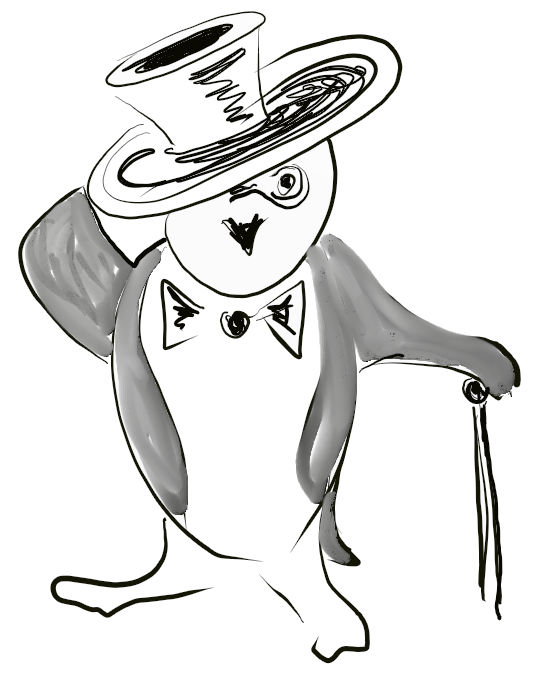
\epsfig{file=picts/gplt3/hat1, width=.27\textwidth}
\end{wrapfigure}
Циклы и макросы в \gplt{} предназначены для создания серий сложных рисунков за один запуск утилиты, показа анимации и т.д.
Кроме показа анимации, основная мотивация для введения циклов и макросов в \gplt{} все та же~--- {\it никакая информация не должна вводиться в компьютер дважды}.
Необходимость дублировать ввод информации неизбежно увеличивает трудозатраты и приводит к ошибкам.

Сразу заметим, что описываемые дальше возможности
изменяют входную последовательность аргументов командной строки \gplt~--- сначала при запуске \gplt{} производятся подстановка макросов и
раскрутка циклов, а уже затем вступает в действие все, что писалось о \gplt{} ранее. Естественно, при этом
в .\gplt-файлы, генерируемые вместе с рисунками, не попадают никакие макросы и циклы, а попадают только результаты их работы.
Чуть менее естественно и очевидно то, что
макросы и циклы не будут действовать из .\gplt-файлов если их включать при помощи опции \verb'-i'.
\footnote{Вы можете вставлять фрагменты кода с макросами и циклами средствами шелл, но это не очень хорошая идея. Если Вы и правда хотите такого~---
хорошо подумайте, скорее всего Вы что-то делаете не так.}
Для упрощения отладки, опция \verb'-debug' перед набором команд для \gnuplot{} показывает
последовательность аргументов командной строки \gplt{} после всех подстановок.

Описанный далее механизм обработки аргументов командной строки можно трактовать как факторизацию~--- есть некоторая последовательность строк,
нужно задать ее при помощи минимального числа символов, используя циклы и макросы. Мы будем называть этот механизм
CLIF\footnote{В альпинизме клифой называется силовая стропа с быстрорегулируемой пряжкой, предназначенная для позиционирования
  альпиниста на стене при движении на искусственных точках опоры (якорных крючьях, шлямбурах, скайхуках и т.д.). Вещь вспомогательная,
  но очень удобная.}
(Command Line Interface Factorization), он доступен в виде отдельного модуля \python3{} в библиотеке \verb'aiwlib' по адресу\\
\url{https://github.com/aivn/aiwlib/blob/master/python3/aiwlib/clif.py}\\
Если Вы хотите отключить CLIF в \gplt, укажите \verb'clif=no' в конфигурационном файле \verb'~/.gplt3'.

CLIF получает на вход список строк (как правило, аргументов командной строки) и возвращает преобразованный список строк.
В CLIF есть пространство имен (словарь), в котором находятся переменные и макросы. Макрос это всегда список значений, при подстановке макрос
преобразуется во фрагмент выходной последовательности (несколько значений). Переменная это всегда одно значение (целое число, число с плавающей точкой или строка).
При подстановке макроса или раскрутке тела цикла создается новое пространство имен, наследующее пространство имен более высокого уровня, т.е. реализован стек.
Все изменения в пространстве имен на текущем кадре стека не видны на вышележащих кадрах стека, т.е. переменные и макросы имеют область видимости.

Имена переменных, счетчиков циклов и макросов должны быть идентификаторами,
т.е. должны состоять из латинских букв, цифр и знаков подчеркивания, не могут начинаться с цифр.

Для задания переменных используется два варианта синтаксиса:
\begin{enumerate}
\item \verb'name#=value' ~--- просто задает значение переменной в текущей области видимости.
\item \verb'name:=value' ~--- задает значение переменной в текущей области видимости и сразу же подставляет ее значение, т.е. в выходную
  последовательность будет добавлено значение \verb'value'. Это прямой аналог операции \verb':=' <<морж>>, введенной в \python.8  (значок и правда похож на моржа).
\end{enumerate}

Макросы подчиняются следующим правилам:
\begin{enumerate}
\item  Для задания макроса используется синтаксис
\verb'name{  ...  body ... }'
Фигурные скобки обрамляют тело макроса, открывающая скобка пишется после имени макроса {\bf слитно, и после нее следует пробел},
закрывающая скобка {\bf обрамляется пробелами}. С точки зрения шелл, передающего аргументы командной строки в \gplt, \verb'name{'
  и \verb'}' должны быть отдельными аргументами командной строки, тело макроса это список~--- последовательность аргументов командной строки, заключенная между ними.
\item Тело макроса может содержать циклы или определения других макросов/переменных, но не может содержать незакрытые \verb'{' или некомплектные закрывающие \verb'}'~---
это очевидное ограничение синтаксиса. Попытка добавить лишнюю \verb'{' продлит тело макроса до конца последовательности аргументов командной строки,
попытка вставить лишнюю закрывающую \verb'}' в тело макроса ограничит тело макроса этой скобкой. 
\item Макросы и переменные могут переопределяться в любой момент времени, в т.ч. макрос может быть переопределен как переменная и наоборот.
Команда \verb'name{ }' создаст пустой макрос.  Для уничтожения макроса или переменной используется синтаксис \verb'name{}' (фигурные скобки без пробела).
\end{enumerate}

Циклы подчиняются следующим правилам:
\begin{enumerate}
\item Для создания цикла используется синтаксис
\begin{verbatim}
counter#  ...  counter sequence ... { ... body ... }
\end{verbatim}
Как и в случае с макросами, с точки зрения шелл \verb'counter#', \verb'{' и \verb'}' должны быть отдельными аргументами.
\item В качестве элементов значения счетчика могут выступать произвольные величины или {\bf результаты подстановки макросов}.
\item В теле цикла доступно значение счетчика (по имени) и номер итерации цикла как \verb'_counter' (к имени счетчика спереди добавляется знак подчеркивания).
\item В теле цикла могут содержаться другие циклы, определения макросов и переменных.
\end{enumerate}

При задании очередного значения счетчика цикла или переменной (счетчик это та же переменная, автоматически изменяющаяся от итерации к итерации цикла)
используется следующий алгоритм:
\begin{enumerate}
\item по возможности значение приводится к типу \verb'int';
\item иначе, если возможно, значение приводится к типу \verb'float';
\item иначе значение остается строкой.
\end{enumerate}
Такой подход позволяет задавать в качестве значений переменных числа и выполнять над ними арифметические операции при подстановке.

Наибольший интерес и сложность представляют подстановки значений макросов и переменных. Здесь основным понятием является словарь со значениями
переменных и макросами, отвечающий текущему кадру стека. 
Каждый раз, когда производится подстановка макроса или разворачивание цикла, создается новый кадр стека с новым словарем переменных и макросов.

Для подстановки макроса используется синтаксис \verb'{name}', на это место подставляется тело макроса как последовательность аргументов командной строки.
Можно указывать отдельные элементы (по номеру) или фрагменты тела макроса (как срез списка) в синтаксисе \python:
\begin{verbatim}
... A{ a b c d }  {A} {A[1]} {A[2:-1]} ...
\end{verbatim}
даст в итоге
\begin{verbatim}
... a b c d   b   c d ...
\end{verbatim}
В теле макроса могут быть подстановки других макросов, но во избежание бесконечной рекурсии сам макрос при подстановке в себя трактуется как
одноименная переменная.

Подстановка переменных для каждого элемента входной последовательности производится один и только один раз.
При подстановке используется метод \verb'str.format' и синтаксис \python{} со следующими расширениями, речь идет об обработке одного токена (включения в фигурные скобки):
\begin{enumerate}
\item если при вызове \verb'str.format' подстановка прошла успешно, то на место токена подставляется то, что получилось, например
\begin{verbatim}
a#=1  ...{a}...  ==>   ...1...
\end{verbatim}
\item иначе производится попытка обработать токен при помощи функции \verb'eval' в глобальном словаре модуля \verb'math', например
\begin{verbatim}
a#=1  ...{sin(a)+1}...  ==>   ...1.8414709848078965...
\end{verbatim}  
\item иначе токен остается без изменений, включая обрамляющие фигурные скобки, например
\begin{verbatim}
...{22qwe}...  ==>   ...{22qwe}...
\end{verbatim}    
\end{enumerate}
Важно понимать, что подстановка макроса как \verb'{name}' (возможно с указанием среза) может добавить в выходную последовательность
несколько элементов из тела макроса, подстановка макроса внутри строки как \verb'...{name}...' всегда добавляет в выходную последовательность только один элемент.

В заключение приведем простейший пример с запуском анимации. Пусть результаты хранятся в пронумерованных файлах \verb'dat/0000.dat' ... \verb'0099.dat'
\begin{verbatim}
$ gplt3 -p .1 i# dat/????.dat { {i} -to '' }
\end{verbatim}
Опция \verb'-p .1' задает паузу между кадрами в 0.1 секунду, счетчик \verb'i' пробегает по всем именам файлов, в теле цикла указывается очередной файл
для отрисовки и производится отрисовка на экран при помощи опции \verb|-to ''|. Такого же эффекта можно было бы достичь, набрав команду
\begin{verbatim}
$ gplt3 -p .1 dat/0000.dat -to '' dat/0001.dat -to ''  dat/0002.dat -to '' ...
\end{verbatim}
но указывать так 100 файлов будет довольно утомительно, кроме того, у шелл есть ограничение на максимальный размер команды.
При сохранении результатов расчетов лидирующие нули в имени файла имеют большое значение~--- шелл упорядочивает файлы лексикографически, т.е. без лидирующих нулей
файл \verb'dat/10.dat' будет идти перед файлом \verb'dat/2.dat'.

Можно записать ролик с анимацией при помощи утилиты \verb'ffmpeg' 
\begin{verbatim}
$ mkdir /tmp/png
$ gplt3 -nav i# dat/????.dat { {i} -to /tmp/png/{_i}.png }
$ ffmpeg -i /tmp/png/%d.png -qscale 1 -r 8 movie.mp4 && rm -rf /tmp/png
\end{verbatim}
Опция \verb'-nav' отключает просмотр сгенерированных рисунков, рисунки сохраняются в директории \verb'/tmp/png' и удаляются после вызова \verb'ffmpeg'.
Рекомендуется сохранять временные файлы именно в поддиректориях \verb'/tmp'~--- для большинства современных дистрибутивов \verb'OS Linux'
это временная директория, смонтированная как файловая система \verb'tmpfs' (фактически оперативная память) с очень высокой скоростью работы.  
Имена файлов с рисунками для \verb'ffmpeg' должны быть пронумерованы с нуля, для этого в аргументе опции \verb'-to' указывается
номер итерации цикла \verb'_i'.

Наконец, при помощи макроса можно, например, <<обратить время вспять>> или вообще закольцевать ролик:
\begin{verbatim}
$ gplt3 -nav M{ dat/????.dat } i# {M} {M[::-1]} { {i} -to /tmp/png/{_i}.png }
\end{verbatim}
Первая подстановка макроса \verb'{M}' добавляет файлы с данными в прямом порядке, вторая подстановка макроса \verb'{M[::-1]}'
при помощи механизма срезов \python{} добавляет файлы с данными в обратном порядке, сформированная последовательность файлов проходится в одном цикле
с общей нумерацией при помощи номера итерации \verb'_i'.
\newpage

\section{Список опций}\label{opt:list:sec}
\begin{wrapfigure}[2]{t}{.3\textwidth}
  \vphantom{.}
  \vspace{-3cm}

  
\epsfig{file=picts/gplt3/read, width=.27\textwidth}
\end{wrapfigure}
В этом разделе приводится полный список опций \gplt{} c их краткими описаниями, раздел фактически дублирует команду \verb'gplt3 -h'.

\begin{itemize}
\item \verb'-h [<gnuplot keywords> or <gplt3 options>]' --- вывод справки \gnuplot{} и/или \gplt, 
  подразделы справки gnuplot можно указывать через точку, квадратные скобки обозначают {\bf не} обязательный фрагмент.
\item \verb'-fn <function>[@<attrs>]' --- добавляет функцию для отрисовки.
\item \verb'-U|-u "<expr>[@<attrs>] ..."' --- выражения для отрисовки из последующих файлов.
\item \verb'<filename>[@<attrs>]' --- добавляет кривые из файла согласно -U или y(x)/z(x,y), один и тот же файл можно
  указывать многократно, но его заголовок будет прочитан только один раз. К указанным ранее файлам можно обращаться
  через номера (все указанные файлы трактуются как список в порядке задания) в виде \verb'[<number-of-file>]', можно задавать
  срезы в синтаксисе \python. Файл добавляется в список только при первом указании (включая стандатный ввод), т.е. опция \verb'[:]' будет
  вставлять каждый раз все файлы по одному разу.
\item \verb'-[std][@<attrs>]' --- прочитает файл с данными со стандартного ввода, опция может использоваться многократно. но реальное чтение данных
  будет произведено только один раз.
\item \verb'-def <name>[(<args>)]=[<expr>]' --- добавляет (или убирает если нет \verb'<expr>')
новое выражение (или функцию если заданы \verb'<args>') в глобальное пространство имен. Позволяет задавать 
многократно используемые выражения или функции. Задаваемые через \verb'-def' выражения и функции
обрабатываются для каждой кривой заново и могут содержать зависимости от метаданных из 
заголовков файлов и \verb'.RACS'. 
В отличии от макросов, \verb'-def' работает из \verb'.gplt3' файлов включаемых через опцию \verb'-i'.
\item \verb:-to <filename>.png|pdf[@<termopts>]|': --- строит график (-to '' на экран)
    и продолжает разбор аргументов, выключает multiplot. 
\item \verb'-nav' --- отключает автоматический просмотр файлов с рисунками, построенными -to.                     
\item \verb'-lb{x,y,z,x2,y2,cb} [<text>][@<offset>,r<degree>,<color>]' --- подписи к осям.
\item \verb'-ttl <text>' --- set title <text>, титульная надпись над рисунком.
\item \verb'-r{x,y,z,x2,y2,cb,t,u,v} [<min>]:[<max>]' --- задает пределы отрисовки.
\item \verb'-[h]3d|-2d' --- включает/выключает 3D режим, -h3d дополнительно включает hidden3d.
\item \verb'-[n]pm3d' --- [un]set pm3d map[; set hidden3d], в[ы]ключает режим pm3d.
\item \verb'-pal <name>[=<values>]' --- устанавливает палитру для режима pm3d.
\item \verb:-ln [x][y][z][x2][y2][c]|'': --- логарифмический масштаб по указанным осям.
\item \verb'-tc{x,y,z,x2,y2,cb} <opts>'  --- настройка тиков (чиселок) по осям, '' выключает,
             @ задает format \verb'"%g"', по осям x2 и y2 тики включаются автоматически. 
\item \verb'-sz <sizeopt>' ---  set size <sizeopts>, размеры графика. 
\item \verb'-sk <keyopt>' --- set key <keyopt>, настройки легенды (ключей).
\item \verb'-nk' --- убирает легенду (ключи). 
\item \verb'-w|-ds <data-style>'  --- стиль данных для следующих кривых, перекрывается \verb'@<attrs>'.
\item \verb'-[n]par' --- включает/выключает параметрический режим.
\item \verb'-[i]smpl|-is <samle1>[,<sample2>]' --- устанавливает [iso]samples (число отсчетов), 
  \verb'-is' устанавливает сразу samples и isosamples.
\item \verb'-sm <opts>' --- set smooth <opts>, устанавливает сглаживание.
\item \verb'-arw [<tag>#]<from>:<to>[@opts]' или \verb'[<tag>#]<from>:<len>:<angle>[@opts]' --- рисует стрелку,
  координаты \verb'<from>' и \verb'<to>' задаются через запятую.
\item \verb'-lbl [<tag>#]<pos>:<text>[@<attrs>]' --- добавляет текстовую метку в точке \verb'<pos>'
   дополнительные атрибуты \verb'<attrs>' трактуются так же как и у подписей к осям.
\item \verb'-o <subplot-pos>' --- автоматически включает режим мультиплот и задает origin 
   следующего графика, закрывается опцией -to или автоматически.
\item \verb'-p <time>' --- задает паузу после построения графика при выводе на экран.
\item \verb'-sv <viewopts>' --- set view <viewopts>, ориентация 3D графика.
\item \verb'-[n]sixel' --- [un]set term [sixelgd], для удаленной работы (работает из mlterm).
\item \verb'-debug' --- режим отладки, вместо gnuplot управляющие инструкции пишутся на stdout.
\item \verb'-dump-config-file' --- создает шаблон ~/.gplt3 для последующего редактирования.
\item \verb'-[u]s <opts>' --- [un]set <opts>, "сырой" ввод в gnuplot, для остальных опций.
\item \verb'-raw <command>' --- отправляет <command> в gnuplot, для остальных опций.
\item \verb'-i <filename>' --- вставляет в опции командной строки содержание файла <filename>
   каждая строка трактуется как набор опций без аргументов (например, -nk -3d), 
   включая имена файлов с данными, или как одна опция с аргументом (-U x**2 x+y)
   аргумент это весь остаток строки; пустые и начинающиеся с \# строки игнорируются.
\item \verb'-[no-]tex-num' --- отключает/включает преобразование чисел с плавающей точкой к дробям \LaTeX.
\end{itemize}

\newpage
\section{Примеры и некоторые рецепты использования}
\begin{wrapfigure}[7]{t}{.3\textwidth}
  \vphantom{.}
  \vspace{-1cm}

  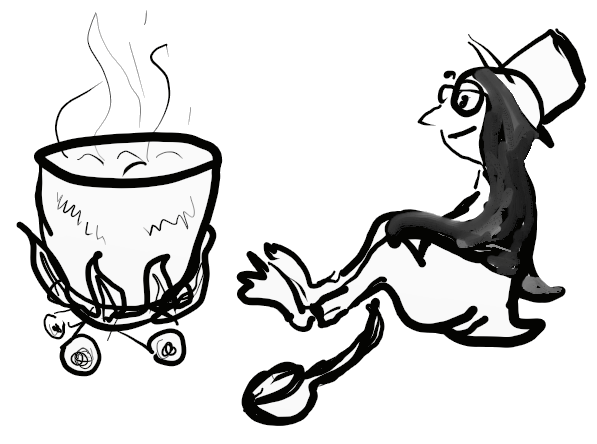
\epsfig{file=picts/gplt3/cook, width=.27\textwidth}
\end{wrapfigure}
В этом разделе собраны типичные примеры использования \gplt.
Для каждого примера приведены команда для запуска \gplt, сгенерированная им последовательность команд
для \gnuplot{} (получена с помощью опции \verb'-debug') и полученный в итоге рисунок.
Чтобы не делать скриншоты экрана, все рисунки (если не сказано иное в случае генерации \pdf-файла) получены при помощи добавления
опций \verb'-sz .7 -to testXXX.png'. Опция \verb'-sz .7' (или даже \verb'-sz .4') нужна для уменьшения рисунка,
в \gnuplot{} размер задается в некоторых безразмерных <<попугаях>> относительно размера окна по умолчанию.
Для простых графиков размер по умолчанию слишком велик, при вставке двух рисунков рядом текст
в зарамочном оформлении получается слишком мелким. Размеры $0.6\div0.7$ позволяют вставлять два рисунка рядом в типичную полосу набора. 
%Настройка терминала (после имени файла через @) \verb'size .7 crop' задает явно размер рисунка, к сожалению, \gnuplot{}
%не делает этого самостоятельно. Для \pdf{} рисунков, пропускаемых через \LaTeX{}, таких проблем нет. 
Изображение в окне \gnuplot{} без \verb'-sz ...' будет отличаться только большими размерами.

Символами \verb'#>>>' отмечен фрагмент опций \gplt{} после подстановки всех макросов, далее следуют команды \gnuplot,
это обычный формат вывода опции \verb'-debug'.\\

%%%%%%%%%%%%%%%%%%%%%%%%%%%%%%%%%%%%%%%%%%%%%%%%%%%%%%%%%%%%%%%%%%%%%%%%%%%%%%%%%%%%%%%%%%%%%%%%%%%%%%%%%%
\noindent\rule{.45\textwidth}{1pt}\hfill \raisebox{-.45\height}{\bf № 1.}  \hfill\rule{.45\textwidth}{1pt}

\vspace{3mm}
\noindent
\begin{minipage}[b]{0.19\textwidth}\small
\begin{verbatim}
$ gplt3 -fn x**2 
#>>> -fn 'x**2'
set xlabel 'x'
set ylabel 'x**2'
plot x**2 notitle   
pause -1
\end{verbatim}
\end{minipage}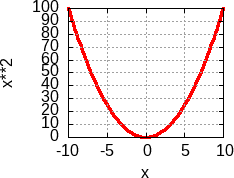
\epsfig{file=picts/gplt3/fig01, width=.25\textwidth}
\hfill
\begin{minipage}[b]{0.27\textwidth}\small
\begin{verbatim}
$ gplt3 -fn x**2 -tcy 20
#>>> -fn 'x**2' -tcy '20'
set ytics 20
set xlabel 'x'
set ylabel 'x**2'
plot x**2 notitle   
pause -1
\end{verbatim}
\end{minipage}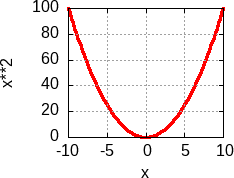
\epsfig{file=picts/gplt3/fig02, width=.25\textwidth}

\vspace{3mm} 

Эти графики построены с опцией \verb'-sz .4', типичной проблемой при малых размерах является налезание тиков (чисел около осей) друг на друга, как на левом графике.
Опция \verb'-tc... '$\delta$ явно задает шаг между тиками.\\


%%%%%%%%%%%%%%%%%%%%%%%%%%%%%%%%%%%%%%%%%%%%%%%%%%%%%%%%%%%%%%%%%%%%%%%%%%%%%%%%%%%%%%%%%%%%%%%%%%%%%%%%%%
\noindent\rule{.45\textwidth}{1pt}\hfill \raisebox{-.45\height}{\bf № 2.}  \hfill\rule{.45\textwidth}{1pt}

%\vspace{3mm}
{\small
\begin{verbatim}
$ gplt3 -fn 'sqrt(1+sin(x)**2)' -fn 'sin(|%x//2%|)**2//2' -sz 1.,.5 -tcy .5 -lby '' \
                                    -sk 'lmargin spacing 2' -to picts/gplt3/fig03.pdf
#>>> -fn 'sqrt(1+sin(x)**2)' -fn 'sin(|%x//2%|)**2//2' -sz '1.,.5' -tcy '.5' -lby '' 
                                 -sk 'lmargin spacing 2' -to 'picts/gplt3/fig03.pdf'
set term epslatex 
set out "/tmp/gplt3-2976974-p.eps"
set size 1.,.5
set ytics .5
set key lmargin spacing 2
set xlabel '$x$'
unset ylabel
plot sqrt(1+sin(x)**2) title '$\sqrt{{1}+{\sin^{2}{x}}}$'  lw 3 , \
 sin(abs(x/2))**2/2 title '$\frac{\sin^{2}{\left|\frac{x}{2}\right|}}{2}$'  lw 3 
set out
!epstopdf --outfile /tmp/gplt3-2976974-p.pdf /tmp/gplt3-2976974-p.eps;        \
          (cd /tmp; pdflatex /tmp/gplt3-2976974.tex | grep \!);               \
          pdfcrop -m 0 /tmp/gplt3-2976974.pdf picts/gplt3/fig03.pdf > /dev/null
!rm -f /tmp/gplt3-2976974.* /tmp/gplt3-2976974-p.*
!evince 'picts/gplt3/fig03.pdf'
\end{verbatim}
  }
\begin{figure}
  \begin{center}
  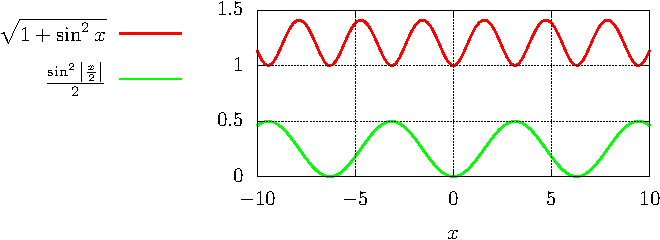
\epsfig{file=picts/gplt3/fig03}
\end{center}
\end{figure}
\noindent
В \gplt{} большое внимание уделяется выводу выражений в формате \LaTeX{} (обратите внимание на задание модуля, дроби и степень функции $\sin$).
В данном случае автоматически сгенерированная метка по оси $y$ оказывается слишком громоздкой, и ее лучше отключить опцией \verb|-lby ''|.
Кроме проблем с налезающими друг на друга подписями к тикам регулярно возникают проблемы с легендой~--- нежелательно, чтобы легенда
перекрывалась кривыми на графике. Если на графике нет свободного места, легенду можно вынести за пределы графика командами \verb'-sk out' (направо)
или, как в этом примере, \verb'-sk lmargin'. Еще одной проблемой с легендой является слишком маленькое расстояние между подписями к кривым,
для ее решения служит опция \verb'-sk spacing 2'. Кроме построения графика с правильными подписями к осям и легендой дополнительная работа
требуется для конвертации пары файлов \verb'eps' и \verb'tex' в \pdf~--- это не обязательно, но значительно упрощает последующую вставку рисунка
в \LaTeX. В \gplt{} все временные файлы для такой конвертации, включая вызов \verb'pdflatex', происходят в файловой системе \verb'tmpfs',
что значительно ускоряет работу.\\

%%%%%%%%%%%%%%%%%%%%%%%%%%%%%%%%%%%%%%%%%%%%%%%%%%%%%%%%%%%%%%%%%%%%%%%%%%%%%%%%%%%%%%%%%%%%%%%%%%%%%%%%%%
\noindent\rule{.45\textwidth}{1pt}\hfill \raisebox{-.45\height}{\bf № 3.}  \hfill\rule{.45\textwidth}{1pt}

%\vspace{3mm}
{\small
\begin{verbatim}
$ gplt3 -sz 1.2,.5                                                              \
        -o 0,0 -sz 'square .5' -par -rt 0:30 -rx -1:1 -ry -1:1                  \
        -fn 'sin(t)*exp(-.1*t),cos(t)*exp(-.1*t)' -lbx x -lby v@2               \
        -o 0.4,0 -sz 'nosquare .65,.5' -lbx t -lby '' -npar -rx 0:30            \
        -fn 'sin(x)*exp(-.1*x)@=x' -fn 'cos(x)*exp(-.1*x)@=v'                   \
        -to picts/gplt3/fig04.pdf 
#>>> -sz '1.2,.5' -o '0,0' -sz 'square .5' -par -rt '0:30' -rx '-1:1' -ry '-1:1' 
     -fn 'sin(t)*exp(-.1*t),cos(t)*exp(-.1*t)' -lbx 'x' -lby 'v@2' -o '0.4,0' 
      -sz 'nosquare .65,.5' -lbx 't' -lby '' -npar -rx '0:30' -fn 'sin(x)*exp(-.1*x)@=x' 
      -fn 'cos(x)*exp(-.1*x)@=v' -to 'picts/gplt3/fig04.pdf'
set term epslatex 
set out "/tmp/gplt3-2979451-p.eps"
set multiplot
set size 1.2,.5
set origin 0,0
set size square .5
set parametric
set trange [0:30]
set xrange [-1:1]
set yrange [-1:1]
set xlabel '$x$'
set ylabel '$v$' offset 2
plot sin(t)*exp(-0.1*t), cos(t)*exp(-0.1*t) notitle  lw 3 
set origin 0.4,0
set size nosquare .65,.5
unset parametric
set xrange [0:30]
set xlabel '$t$'
unset ylabel
plot sin(x)*exp(-0.1*x) title "$x$"  lw 3 , cos(x)*exp(-0.1*x) title "$v$"  lw 3 
unset multiplot
set out
!epstopdf --outfile /tmp/gplt3-2979451-p.pdf /tmp/gplt3-2979451-p.eps;        \
          (cd /tmp; pdflatex /tmp/gplt3-2979451.tex | grep \!);               \
          pdfcrop -m 0 /tmp/gplt3-2979451.pdf picts/gplt3/fig04.pdf > /dev/null
!rm -f /tmp/gplt3-2979451.* /tmp/gplt3-2979451-p.*
!evince 'picts/gplt3/fig04.pdf'\end{verbatim}
  }

  \begin{center}
  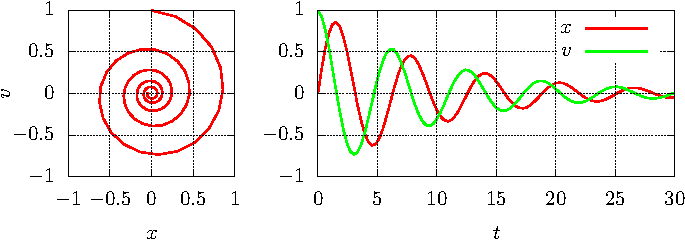
\epsfig{file=picts/gplt3/fig04}
\end{center}
В этом примере задействован режим \verb'multiplot', обратите внимание на опцию \verb'-o' и расположение опций \verb'-sz'~---
первая \verb'-sz 1.2,.5' задает размер всего графика в целом, остальные две задают размеры графиков внутри \verb'multiplot'.
Опция \verb'-lby v@2' задает подпись $v$ по оси $y$ и сдвигает ее на две условных единицы (порядка размера символа) ближе к оси. Опции \verb'-par' и \verb'-npar'
включают и выключают параметрический режим. Опциии \verb'-rx -1:1' и т.д. задают пределы по различным осям. Атрибуты \verb'@=x' и  \verb'@=v' в конце функций
задают подписи к кривым на легенде.
Несмотря на всю лаконичность \gplt, построение сложных графиков все еще остается непростой задачей, но сравните~--- сколько всего пришлось бы писать для \gnuplot!
При работе с файлами команды для \gplt{}, как правило, оказываются короче, чем при задании  аналитических функций.\\

\newpage
%%%%%%%%%%%%%%%%%%%%%%%%%%%%%%%%%%%%%%%%%%%%%%%%%%%%%%%%%%%%%%%%%%%%%%%%%%%%%%%%%%%%%%%%%%%%%%%%%%%%%%%%%%
\noindent\rule{.45\textwidth}{1pt}\hfill \raisebox{-.45\height}{\bf № 4.}  \hfill\rule{.45\textwidth}{1pt}

%\vspace{3mm}
{\small
\begin{verbatim}
$ gplt3 -h3d -fn 'f:=sin(x)*cos(y)@1' -is 100 -sz .7 -lbz @1,r90 -tcz .5 \
         -to picts/gplt3/fig05.png  -tccb .5 -pm3d -sz square  -fn {f}   \
         -to picts/gplt3/fig06.pdf -debug
#>>> -h3d -fn 'sin(x)*cos(y)@1' -is '100' -sz '.7' -lbz '@1,r90' -tcz '.5' 
      -to 'picts/gplt3/fig05.png'
set term png 
set out "/tmp/gplt3-2981753.png"
set hidden3d
set samples 100
set isosamples 100
set size .7
set ztics .5
set xlabel 'x'
set ylabel 'y'
set zlabel 'sin(x)*cos(y)' offset 1 rotate by 90
splot sin(x)*cos(y) notitle  lw 1
set out
!convert /tmp/gplt3-2981753.png -trim 'picts/gplt3/fig05.png' &&  \
         rm /tmp/gplt3-2981753.png
!qiv 'picts/gplt3/fig05.png'
#>>> -tccb '.5' -pm3d -sz 'square' -fn 'sin(x)*cos(y)@1' 
     -to 'picts/gplt3/fig06.pdf'
set term epslatex 
set out "/tmp/gplt3-2981753-p.eps"
set cbtics .5
set hidden3d
set pm3d map
set size square
set xlabel '$x$'
set ylabel '$y$'
set cblabel '$\sin{x}\,\cos{y}$'
splot sin(x)*cos(y) notitle  lw 1
set out
!epstopdf --outfile /tmp/gplt3-2981753-p.pdf /tmp/gplt3-2981753-p.eps; \
   (cd /tmp; pdflatex /tmp/gplt3-2981753.tex | grep \!); \
   pdfcrop -m 0 /tmp/gplt3-2981753.pdf picts/gplt3/fig06.pdf > /dev/null
!rm -f /tmp/gplt3-2981753.* /tmp/gplt3-2981753-p.*
!evince 'picts/gplt3/fig06.pdf'
\end{verbatim}
}
\begin{center}
  \begin{tabular}{cc}
    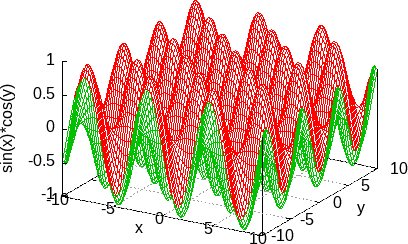
\epsfig{file=picts/gplt3/fig05, width=.5\textwidth} & 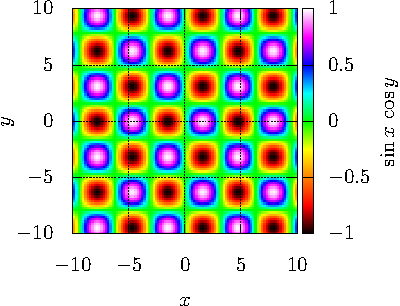
\epsfig{file=picts/gplt3/fig06}
  \end{tabular}
\end{center}
Это пример использования <<моржового>> оператора \verb':=' для задания переменной в \gplt~--- функция для отрисовки используется повторно.
Один вызов \gplt{} создает сразу два графика с одной и той же функцией, но в разном представлении.
Толщина линии специально явно задана в 1px, линии в 3px на таком графике сольются. 
Обычные трехмерные графики (слева) плохо подходят для вставки в печатные работы (на бумаге график статичен,
при отображении на экране график можно покрутить), цветная визуализация с хорошей палитрой
гораздо информативнее (режим \verb'-pm3d', справа). Обратите внимание на поворот и сдвиг подписи по оси $z$ на графике слева опцией \verb'-lbz  @1,r90'
без явного задания текста подписи.
В этом примере не пришлось вручную править текст подписей к осям.\\

%%%%%%%%%%%%%%%%%%%%%%%%%%%%%%%%%%%%%%%%%%%%%%%%%%%%%%%%%%%%%%%%%%%%%%%%%%%%%%%%%%%%%%%%%%%%%%%%%%%%%%%%%%
\noindent\rule{.45\textwidth}{1pt}\hfill \raisebox{-.45\height}{\bf № 5.}  \hfill\rule{.45\textwidth}{1pt}

\vspace{3mm}
Создадим два тестовых файла:
{\small
\begin{verbatim}
$ python3 -c 'import random; print("#:omega0 beta err\n"+"".join("%g %g %g\n"%(i,    \
  i**.5+random.normalvariate(0,.1),random.normalvariate(0,.5)) for i in range(20)))' \
  > dat/test1.dat
$ cat dat/test1.dat
#:omega0 beta err
0 0.0742779 -1.04481
1 0.953205 0.202459
...
$ python3 -c 'from math import *; print("#:t E.x E.y E.z H[] H[] H[]\n"+             \
  "".join("%g %g 0 0 0 %g 0\n"%(i*.1, sin(i*.1), cos(i*.1)) for i in range(200)))'   \
  > dat/test2.dat
$ cat dat/test2.dat
#:t E.x E.y E.z H[] H[] H[]
0 0 0 0 0 0 0
0.1 0.0998334 0 0 0 0.0998334 0
...
\end{verbatim}
}
В первом файле лежат данные гипотетического расчета, во втором плоская электромагнитная волна, распространяющаяся
вдоль оси $z$. В заголовке второго файла столбцы проименованы как вектора ${\bf E}=(E_x, E_y, E_z)$ и ${\bf H}=(H_0, H_1, H_2)$ в двух разных форматах.\\

\noindent
\begin{minipage}[b]{.69\textwidth}
  \small
\begin{verbatim}
$ gplt3 dat/test1.dat  -debug
#>>> dat/test1.dat
set xlabel 'omega0'
set ylabel 'beta'
plot 'dat/test1.dat' u (($1)):(($2)) notitle   
pause -1
\end{verbatim}
\end{minipage}
\raisebox{-1.1cm}{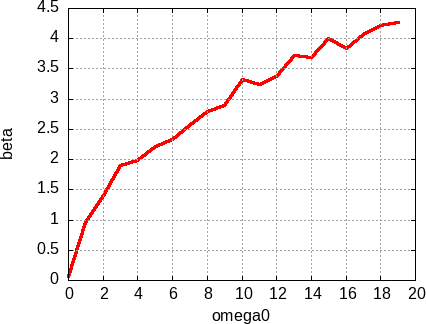
\epsfig{file=picts/gplt3/fig07, width=.3\textwidth}}
\begin{minipage}[b]{.54\textwidth}
  \small
\begin{verbatim}
$ gplt3 dat/test?.dat -sz .6 -to picts/gplt3/fig08.pdf
#>>> dat/test1.dat dat/test2.dat -sz '.6' -sk 'left' -to 'picts/gplt3/fig08.pdf'
set term epslatex 
set out "/tmp/gplt3-3090408-p.eps"
set size .6
set key left
set xlabel '$\omega_{0}$, $t$'
set ylabel '$\beta$, $E_{x}$'
plot 'dat/test1.dat' u (($1)):(($2)) title \
  '...1: $\beta$'  lw 3 , 'dat/test2.dat'  \
  u (($1)):(($2)) title '...2: $E_{x}$'  lw 3 
set out
!epstopdf --outfile /tmp/gplt3-3090408-p.pdf   \
  /tmp/gplt3-3090408-p.eps; (cd /tmp; pdflatex \
  /tmp/gplt3-3090408.tex | grep \!); pdfcrop    \
  -m 0 /tmp/gplt3-3090408.pdf picts/gplt3/fig08.pdf > /dev/null
\end{verbatim}
\end{minipage}
\raisebox{.5cm}{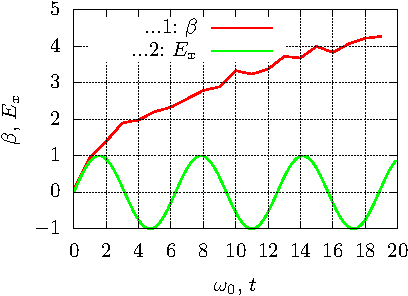
\epsfig{file=picts/gplt3/fig08, width=.45\textwidth}}
\begin{verbatim}
!rm -f /tmp/gplt3-3090408.* /tmp/gplt3-3090408-p.*
!evince 'picts/gplt3/fig08.pdf'
\end{verbatim}

%\vspace{5mm}
При отрисовке файлов \gplt{} извлекает из заголовков имена столбцов и автоматически формирует подписи к осям и легенду.
По умолчанию, в зависимости от режима (\verb'-2d' или \verb'-3d') рисуются первые $2\div3$ столбца.
Если в легенде указываются имена файлов,
то они сокращаются до необходимого минимума. При выводе в \pdf{}, по возможности, для имен столбцов формируются корректные имена \LaTeX.
Иногда приходится вручную позиционировать легенду (например, \verb'-sk left') так, чтобы она не пересекалась с кривыми.\\

%%%%%%%%%%%%%%%%%%%%%%%%%%%%%%%%%%%%%%%%%%%%%%%%%%%%%%%%%%%%%%%%%%%%%%%%%%%%%%%%%%%%%%%%%%%%%%%%%%%%%%%%%% 
\noindent\rule{.45\textwidth}{1pt}\hfill \raisebox{-.45\height}{\bf № 6.}  \hfill\rule{.45\textwidth}{1pt}

\vspace{3mm}
\noindent
\begin{minipage}[b]{.59\textwidth}
\small
\begin{verbatim}
$ gplt3 -U omega0,beta,err@errorbars dat/test1.dat 
        -fn 'sqrt(x)' -sk left
#>>> -U 'omega0,beta,err@errorbars' dat/test1.dat 
     -fn 'sqrt(x)' -sk 'left'
set key left
set xlabel 'omega0'
set ylabel 'beta'
plot 'dat/test1.dat' u (($1)):(($2)):(($3))  \
     title 'calc'  with errorbars  , sqrt(x) \
     title 'theor'   
pause -1
\end{verbatim}
\end{minipage}
\raisebox{-0cm}{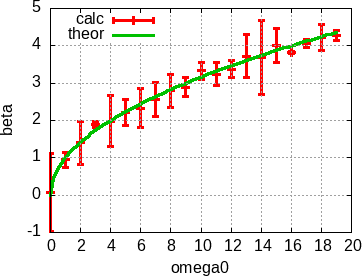
\epsfig{file=picts/gplt3/fig09, width=.4\textwidth}}\\[5mm]
Опция \verb'-U' позволяет явно задавать выражения для отрисовки из файла. По умолчанию выражение строится от первого (или первых двух) столбца,
но ситуацию можно изменить, перечислив выражения для отрисовки через запятую или указав аргументы выражения в скобках. Если стиль
отрисовки требует больше выражений, чем обычно (здесь задана еще величина ошибки), то перечисление через запятую является единственным вариантом.
При построении двух кривых~--- данных из файла и функции~--- в легенде по умолчанию задаются подписи calc и theor.\\

%%%%%%%%%%%%%%%%%%%%%%%%%%%%%%%%%%%%%%%%%%%%%%%%%%%%%%%%%%%%%%%%%%%%%%%%%%%%%%%%%%%%%%%%%%%%%%%%%%%%%%%%%%
\noindent\rule{.45\textwidth}{1pt}\hfill \raisebox{-.45\height}{\bf № 7.}  \hfill\rule{.45\textwidth}{1pt}

\vspace{3mm}
\noindent
\begin{minipage}[b]{.48\textwidth}
\small
\begin{verbatim}
$ gplt3 -U 'E.x@7 H[1]' dat/test2.dat -sz .6 -tcx 5 -tcy .5 -sk 'out samplen 1' \
        -to picts/gplt3/fig10.pdf
#>>> -U 'E.x@7 H[1]' dat/test2.dat -sz '.6' -tcx '5' -tcy '.5' -sk 'out samplen 1' 
     -to 'picts/gplt3/fig10.pdf'
set term epslatex 
set out "/tmp/gplt3-3102156-p.eps"
set size .6
set xtics 5
set ytics .5
set key out samplen 1
set xlabel '$t$'
set ylabel '$E_{x}$, $H_{1}$'
plot 'dat/test2.dat' u (($1)):(($2))     \
  title '$E_{x}$'  lw 7, 'dat/test2.dat' \
  u (($1)):(($6)) title '$H_{1}$'  lw 3 
set out
!epstopdf --outfile /tmp/gplt3-3102156-p.pdf \
/tmp/gplt3-3102156-p.eps; (cd /tmp; pdflatex /tmp/gplt3-3102156.tex | grep \!);  \
  pdfcrop -m 0 /tmp/gplt3-3102156.pdf picts/gplt3/fig10.pdf > /dev/null
!rm -f /tmp/gplt3-3102156.* /tmp/gplt3-3102156-p.*
!evince 'picts/gplt3/fig10.pdf'
\end{verbatim}
\end{minipage}
\raisebox{2cm}{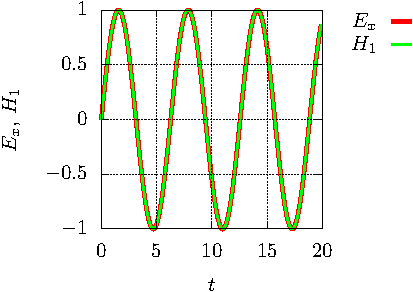
\epsfig{file=picts/gplt3/fig10, width=.5\textwidth}}\\[5mm]
Опция \verb'-U' позволяет в своем аргументе указывать несколько кривых для отрисовки через пробел (в этом случае обязательны кавычки).
По умолчанию зависимости строятся от первого столбца в данном случае времени. В выражениях можно указывать отдельные компоненты векторов.
Если кривые совпадают, чтобы это подчеркнуть, можно первую кривую сделать гораздо толще.
Легенда и тики могут требовать дополнительной настройки, здесь легенда вынесена за пределы графика и уменьшена длина линий на легенде.\\

\newpage
%%%%%%%%%%%%%%%%%%%%%%%%%%%%%%%%%%%%%%%%%%%%%%%%%%%%%%%%%%%%%%%%%%%%%%%%%%%%%%%%%%%%%%%%%%%%%%%%%%%%%%%%%%
\noindent\rule{.45\textwidth}{1pt}\hfill \raisebox{-.45\height}{\bf № 8.}  \hfill\rule{.45\textwidth}{1pt}

\vspace{3mm}
\noindent
\begin{minipage}[b]{.73\textwidth}
\small
\begin{verbatim}
$ gplt3 -U 'E.x(cos(t))' dat/test2.dat -sz square
#>>> -U 'E.x(cos(t))' dat/test2.dat -sz 'square'
set size square
set xlabel 'cos(t)'
set ylabel 'E_x'
plot 'dat/test2.dat' u (cos(($1))):(($2)) notitle   
pause -1
\end{verbatim}
\end{minipage}
\raisebox{-.5cm}{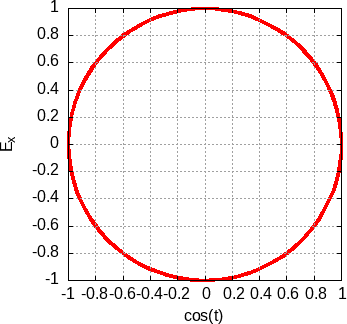
\epsfig{file=picts/gplt3/fig11, width=.25\textwidth}}\\[5mm]
Как уже отмечалось выше, выражение по оси $x$  можно указывать как аргумент выражения откладываемого по оси $y$.

%%%%%%%%%%%%%%%%%%%%%%%%%%%%%%%%%%%%%%%%%%%%%%%%%%%%%%%%%%%%%%%%%%%%%%%%%%%%%%%%%%%%%%%%%%%%%%%%%%%%%%%%%% 
\noindent\rule{.45\textwidth}{1pt}\hfill \raisebox{-.45\height}{\bf № 9.}  \hfill\rule{.45\textwidth}{1pt}

\vspace{3mm}
\noindent
\begin{minipage}[b]{.67\textwidth}
\small
\begin{verbatim}
$ gplt3 -U '|%E%H%|' dat/test2.dat -sz .6 -tcy .2 -to picts/gplt3/fig12.pdf -debug
#>>> -U '|%E%H%|' dat/test2.dat -sz '.6' -tcy '.2' -to 'picts/gplt3/fig12.pdf'
set term epslatex 
set out "/tmp/gplt3-236108-p.eps"
set size .6
set ytics .2
set xlabel '$t$'
set ylabel '$\left|{\mathbf E}\times {\mathbf H}\right|$'
plot 'dat/test2.dat' u (($1)):(sqrt((($3)*($7)-         \
     ($4)*($6))*(($3)*($7)-($4)*($6))+(($4)*($5)-       \
     ($2)*($7))*(($4)*($5)-($2)*($7))+(($2)*($6)-       \
     ($3)*($5))*(($2)*($6)-($3)*($5)))) notitle  lw 3 
set out
!epstopdf --outfile /tmp/gplt3-236108-p.pdf /tmp/gplt3-236108-p.eps;   \
     (cd /tmp; pdflatex /tmp/gplt3-236108.tex | grep \!); pdfcrop -m 0 \
     /tmp/gplt3-236108.pdf picts/gplt3/fig12.pdf > /dev/null
!rm -f /tmp/gplt3-236108.* /tmp/gplt3-236108-p.*
!evince 'picts/gplt3/fig12.pdf'
unset term
\end{verbatim}
\end{minipage}
\raisebox{2.9cm}{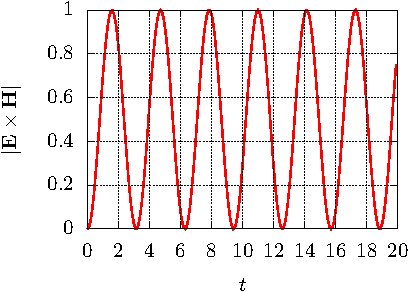
\epsfig{file=picts/gplt3/fig12, width=.33\textwidth}}\\[5mm]
Поддерживаются операции над векторами, в частности векторное произведение (перегруженная операция \verb'%') и модуль от вектора.
Обратите внимание на формат ввода выражения для отрисовки и подпись к оси $y$.
\vspace{3mm}

%%%%%%%%%%%%%%%%%%%%%%%%%%%%%%%%%%%%%%%%%%%%%%%%%%%%%%%%%%%%%%%%%%%%%%%%%%%%%%%%%%%%%%%%%%%%%%%%%%%%%%%%%%
\noindent\rule{.45\textwidth}{1pt}\hfill \raisebox{-.45\height}{\bf № 10.}  \hfill\rule{.45\textwidth}{1pt}

\vspace{3mm}
\noindent
{\small
\begin{verbatim}
$ gplt3 -U 'E+(0,0,t) H+(0,0,t) 0,0,t' dat/test2.dat -3d -lbx x@0,-.5 -lby y@-2,-1 \
          -lbz @2,r90 -tcx '.5 off 0,-.5' -tcy .5 -tcz 5 -to picts/gplt3/fig13.pdf
#>>> -U 'E+(0,0,t) H+(0,0,t) 0,0,t' dat/test2.dat -3d -lbx 'x@0,-.5' -lby 'y@-2,-1' 
    -lbz '@2,r90' -tcx '.5 off 0,-.5' -tcy '.5' -tcz '5' -to 'picts/gplt3/fig13.pdf'
set term epslatex 
set out "/tmp/gplt3-271488-p.eps"
set xtics .5 off 0,-.5
set ytics .5
set ztics 5
set xlabel '$x$' offset 0,-.5
set ylabel '$y$' offset -2,-1
set zlabel '${E_{z}}+{t}$, ${H_{2}}+{t}$, $t$' offset 2 rotate by 90
splot 'dat/test2.dat' u (($2)+0):(($3)+0):(($4)+($1)) title '${E_{z}}+{t}$'  lw 3, \
      'dat/test2.dat' u (($5)+0):(($6)+0):(($7)+($1)) title '${H_{2}}+{t}$'  lw 3, \
      'dat/test2.dat' u (0):(0):(($1)) title '$t$'  lw 3 
set out
!epstopdf --outfile /tmp/gplt3-271488-p.pdf /tmp/gplt3-271488-p.eps;               \
    (cd /tmp; pdflatex /tmp/gplt3-271488.tex | grep \!); pdfcrop -m 0              \
    /tmp/gplt3-271488.pdf picts/gplt3/fig13.pdf > /dev/null
!rm -f /tmp/gplt3-271488.* /tmp/gplt3-271488-p.*
!evince 'picts/gplt3/fig13.pdf'
unset term
\end{verbatim}
  }
\vspace{-1cm}
\begin{center}
\epsfig{file=picts/gplt3/fig13}\\[3mm]
\end{center}
В качестве векторов так же могут выступать кортежи или списки. Точно такой же график можно было бы построить с опцией
\begin{verbatim}
-U '(E.z+t)(E.x,E.y) (H[2]+t)(H[0],H[1]) 0,0,t'
\end{verbatim}
или
\begin{verbatim}
-U 'E.x,E.y,(E.z+t) H[0],H[1],(H[2]+t) 0,0,t'
\end{verbatim}
При построении трехмерных графиков больше всего сложностей
вызывает корректное расположение подписей к осям и тиков --- к сожалению \gnuplot{} по умолчанию расставляет их плохо, подписи
налезают друг на друга и на рисунок.

\newpage
\section{Заключение}
\begin{wrapfigure}[7]{t}{.3\textwidth}
  \vphantom{.}

  \vspace{-2.3cm}
  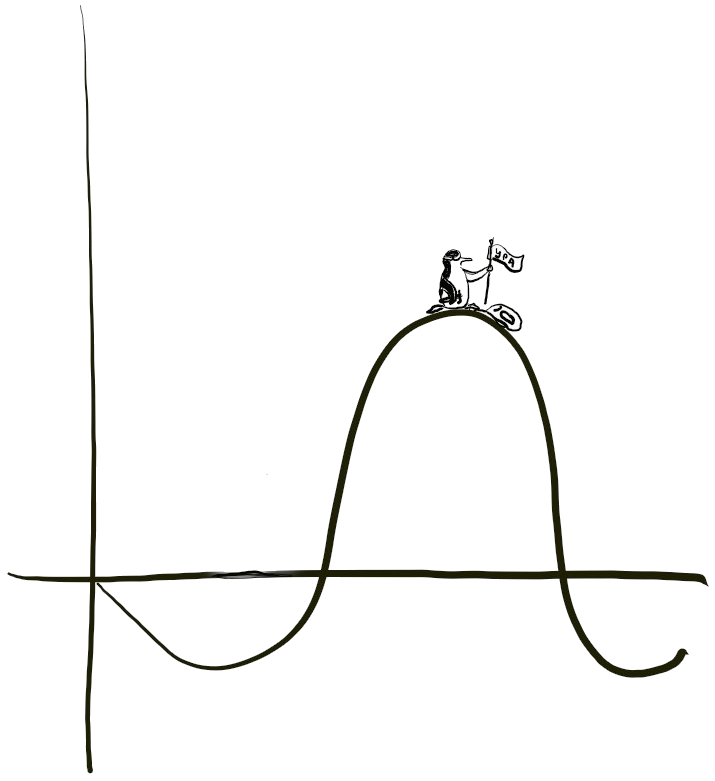
\epsfig{file=picts/gplt3/sin3, width=.27\textwidth}
\end{wrapfigure}

Трудно сказать, почему некоторые утилиты или языки программирования получают всеобщее признание, несмотря на все свои недостатки,
а другие, будучи близкими к идеалу, остаются в забвении. 
Утилита \gplt{}, конечно, не идеальна, она писалась <<для себя>>, под специфические запросы автора.
Подготовка рисунков для статей это всегда большая и кропотливая работа~---
абсолютное большинство рисунков для своих статей за последние 15 лет сделаны автором в \verb'gplt' различных версий.

Ключевым недостатком предыдущих версий \verb'gplt' являлось отсутствие подробной документации,
\verb'gplt' использовали в основном некоторые из коллег, бывшие студенты автора, познакомившиеся с \verb'gplt'
в процессе обучения. Для \gplt{}  этот недостаток, наконец, исправлен. 

\bibliographystyle{myugost2008}
\bibliography{lit}

\appendix\section{Обновления}
Поскольку это руководство оказалось достаточно объемным, а утилита \gplt{} продолжает развиваться, был создан раздел содержащий краткое описание обновлений
в хронологическом порядке. Предыдущие разделы руководства поддерживаются в актуальном состоянии, так что если Вы прочитали последнюю версию руководства
(дата указана на титульной странице)~--- Вы в курсе текущего состояния дел. Если же вы читали старую версию, Вам достаточно найти в этом разделе
соответствующую дату и прочитать от нее и до конца, что бы ознакомиться с произошедшими с того момента изменениями.

\paragraph{16 декабря 2023.} Реализована возможность обращения к файлам с данными по номерам через квадратные скобки, включая срезы,
см. раздел~\ref{main:sec}. Добавлены функции $\min$, $\max$ и \verb'atan2'. Добавлены опции \verb'-arw' (рисование стрелок) и \verb'-lbl' (добавляет текстовые метки),
см. раздел~\ref{opt:list:sec}.
В документацию добавлены примеры №$9, 10$ посвященные работе с векторами из заголовка файла.

\paragraph{18 декабря 2023.} Добавлена поддержка фильтров (\verb'bash' команд пишушщих данные на стандартный вывод), сжатых \verb'.gz' файлов  и \verb'.csv' файлов.
Для задания фильтра надо указать вначале \verb'!', например \verb|gplt3 '!echo  "1 2\n3 4"'|.
При работе с \verb'.csv'-файлами опционально заголовок может занимать первую строчку и содержать только имена столбцов. Никакой символ комментирования не требуется,
имена столбцов идут через тот же разделитель что и весь остальной файл~--- разделитель \verb';' или \verb',', для всего файла раздилетль должен быть один и тот же.
Первая строка трактуется как заголовок если первый элемент первой строки не может быть приведен к \verb'float'.
Векторные имена столбцов для \verb'.csv' не поддерживаются. 


\paragraph{24 декабря 2023.} Добавлена опция \verb'-def <name>[(<args>)]=[<expr>]'. Опция добавляет (или убирает если нет \verb'<expr>')
новое выражение (или функцию если заданы \verb'<args>') в глобальное пространство имен. Позволяет задавать 
многократно используемые выражения или функции. Задаваемые через \verb'-def' выражения и функции
обрабатываются для каждой кривой заново и могут содержать зависимости от метаданных из 
заголовков файлов и \verb'.RACS'. 
В отличии от макросов, \verb'-def' работает из \verb'.gplt3' файлов включаемых через опцию \verb'-i'.

Добавлена функция \verb'ifch(<expr1>,<cond1>,<expr2>[,<cond2>,<expr3>,...])' которая трактуется как цепочка
\verb'<expr1> if <cond1> else <expr2> if <cond2> else <expr3> ...'

\paragraph{26 декабря 2023.} Добавлена поддержка факториала и двойного факториала, задаются как \verb'!' и \verb'!!', имеют такой же приоритет как возведение в степень.

\paragraph{17 апреля 2024.} Добавлена возможность перечисления нескольких выражений через запятую в подписях к осям, легендах кривых и титуле. Добавлены опции \verb'-[no-]tex-num', отключающие/включающие преобразование чисел с плавающей точкой к дробям \LaTeX.

\end{document}
